\documentclass[twoside]{book}

% Packages required by doxygen
\usepackage{calc}
\usepackage{doxygen}
\usepackage{graphicx}
\usepackage[utf8]{inputenc}
\usepackage{makeidx}
\usepackage{multicol}
\usepackage{multirow}
\usepackage{textcomp}
\usepackage[table]{xcolor}

% Font selection
\usepackage[T1]{fontenc}
\usepackage{mathptmx}
\usepackage[scaled=.90]{helvet}
\usepackage{courier}
\usepackage{amssymb}
\usepackage{sectsty}
\renewcommand{\familydefault}{\sfdefault}
\allsectionsfont{%
  \fontseries{bc}\selectfont%
  \color{darkgray}%
}
\renewcommand{\DoxyLabelFont}{%
  \fontseries{bc}\selectfont%
  \color{darkgray}%
}

% Page & text layout
\usepackage{geometry}
\geometry{%
  a4paper,%
  top=2.5cm,%
  bottom=2.5cm,%
  left=2.5cm,%
  right=2.5cm%
}
\tolerance=750
\hfuzz=15pt
\hbadness=750
\setlength{\emergencystretch}{15pt}
\setlength{\parindent}{0cm}
\setlength{\parskip}{0.2cm}
\makeatletter
\renewcommand{\paragraph}{%
  \@startsection{paragraph}{4}{0ex}{-1.0ex}{1.0ex}{%
    \normalfont\normalsize\bfseries\SS@parafont%
  }%
}
\renewcommand{\subparagraph}{%
  \@startsection{subparagraph}{5}{0ex}{-1.0ex}{1.0ex}{%
    \normalfont\normalsize\bfseries\SS@subparafont%
  }%
}
\makeatother

% Headers & footers
\usepackage{fancyhdr}
\pagestyle{fancyplain}
\fancyhead[LE]{\fancyplain{}{\bfseries\thepage}}
\fancyhead[CE]{\fancyplain{}{}}
\fancyhead[RE]{\fancyplain{}{\bfseries\leftmark}}
\fancyhead[LO]{\fancyplain{}{\bfseries\rightmark}}
\fancyhead[CO]{\fancyplain{}{}}
\fancyhead[RO]{\fancyplain{}{\bfseries\thepage}}
\fancyfoot[LE]{\fancyplain{}{}}
\fancyfoot[CE]{\fancyplain{}{}}
\fancyfoot[RE]{\fancyplain{}{\bfseries\scriptsize Generated on Tue Aug 19 2014 14\-:56\-:12 for My Project by Doxygen }}
\fancyfoot[LO]{\fancyplain{}{\bfseries\scriptsize Generated on Tue Aug 19 2014 14\-:56\-:12 for My Project by Doxygen }}
\fancyfoot[CO]{\fancyplain{}{}}
\fancyfoot[RO]{\fancyplain{}{}}
\renewcommand{\footrulewidth}{0.4pt}
\renewcommand{\chaptermark}[1]{%
  \markboth{#1}{}%
}
\renewcommand{\sectionmark}[1]{%
  \markright{\thesection\ #1}%
}

% Indices & bibliography
\usepackage{natbib}
\usepackage[titles]{tocloft}
\setcounter{tocdepth}{3}
\setcounter{secnumdepth}{5}
\makeindex

% Hyperlinks (required, but should be loaded last)
\usepackage{ifpdf}
\ifpdf
  \usepackage[pdftex,pagebackref=true]{hyperref}
\else
  \usepackage[ps2pdf,pagebackref=true]{hyperref}
\fi
\hypersetup{%
  colorlinks=true,%
  linkcolor=blue,%
  citecolor=blue,%
  unicode%
}

% Custom commands
\newcommand{\clearemptydoublepage}{%
  \newpage{\pagestyle{empty}\cleardoublepage}%
}


%===== C O N T E N T S =====

\begin{document}

% Titlepage & ToC
\hypersetup{pageanchor=false}
\pagenumbering{roman}
\begin{titlepage}
\vspace*{7cm}
\begin{center}%
{\Large My Project }\\
\vspace*{1cm}
{\large Generated by Doxygen 1.8.5}\\
\vspace*{0.5cm}
{\small Tue Aug 19 2014 14:56:12}\\
\end{center}
\end{titlepage}
\clearemptydoublepage
\tableofcontents
\clearemptydoublepage
\pagenumbering{arabic}
\hypersetup{pageanchor=true}

%--- Begin generated contents ---
\chapter{Hierarchical Index}
\section{Class Hierarchy}
This inheritance list is sorted roughly, but not completely, alphabetically\-:\begin{DoxyCompactList}
\item \contentsline{section}{\-\_\-\-Lib\-Mesh\-Problem}{\pageref{class___lib_mesh_problem}}{}
\begin{DoxyCompactList}
\item \contentsline{section}{Con\-\_\-\-Diff\-Problem}{\pageref{class_con___diff_problem}}{}
\item \contentsline{section}{Laplace\-Problem}{\pageref{class_laplace_problem}}{}
\item \contentsline{section}{Linear\-Elastic\-Problem}{\pageref{class_linear_elastic_problem}}{}
\item \contentsline{section}{Monodim\-\_\-\-Problem}{\pageref{class_monodim___problem}}{}
\item \contentsline{section}{N\-S\-\_\-\-Problem}{\pageref{class_n_s___problem}}{}
\item \contentsline{section}{N\-S\-\_\-\-Problem3\-D}{\pageref{class_n_s___problem3_d}}{}
\end{DoxyCompactList}
\item Equation\-Systems\begin{DoxyCompactList}
\item \contentsline{section}{Equation\-Systems\-Extended}{\pageref{class_equation_systems_extended}}{}
\end{DoxyCompactList}
\item \contentsline{section}{L\-I\-B\-M\-E\-S\-H}{\pageref{class_l_i_b_m_e_s_h}}{}
\item \contentsline{section}{Lib\-Mesh\-Function}{\pageref{class_lib_mesh_function}}{}
\item Node\begin{DoxyCompactList}
\item \contentsline{section}{Node\-Ext}{\pageref{class_node_ext}}{}
\end{DoxyCompactList}
\item \contentsline{section}{node\-Compare}{\pageref{structnode_compare}}{}
\item ofstream\begin{DoxyCompactList}
\item \contentsline{section}{Debug}{\pageref{class_debug}}{}
\end{DoxyCompactList}
\item Parallel\-Mesh\begin{DoxyCompactList}
\item \contentsline{section}{Parallel\-Mesh\-Extended}{\pageref{class_parallel_mesh_extended}}{}
\end{DoxyCompactList}
\item \contentsline{section}{L\-I\-B\-M\-E\-S\-H\-:\-:s\-B\-C}{\pageref{struct_l_i_b_m_e_s_h_1_1s_b_c}}{}
\item \contentsline{section}{Timer}{\pageref{class_timer}}{}
\end{DoxyCompactList}

\chapter{Class Index}
\section{Class List}
Here are the classes, structs, unions and interfaces with brief descriptions\-:\begin{DoxyCompactList}
\item\contentsline{section}{\hyperlink{class___lib_mesh_problem}{\-\_\-\-Lib\-Mesh\-Problem} }{\pageref{class___lib_mesh_problem}}{}
\item\contentsline{section}{\hyperlink{class_con___diff_problem}{Con\-\_\-\-Diff\-Problem} }{\pageref{class_con___diff_problem}}{}
\item\contentsline{section}{\hyperlink{class_debug}{Debug} }{\pageref{class_debug}}{}
\item\contentsline{section}{\hyperlink{class_equation_systems_extended}{Equation\-Systems\-Extended} }{\pageref{class_equation_systems_extended}}{}
\item\contentsline{section}{\hyperlink{class_laplace_problem}{Laplace\-Problem} }{\pageref{class_laplace_problem}}{}
\item\contentsline{section}{\hyperlink{class_l_i_b_m_e_s_h}{L\-I\-B\-M\-E\-S\-H} }{\pageref{class_l_i_b_m_e_s_h}}{}
\item\contentsline{section}{\hyperlink{class_lib_mesh_function}{Lib\-Mesh\-Function} }{\pageref{class_lib_mesh_function}}{}
\item\contentsline{section}{\hyperlink{class_linear_elastic_problem}{Linear\-Elastic\-Problem} }{\pageref{class_linear_elastic_problem}}{}
\item\contentsline{section}{\hyperlink{class_monodim___problem}{Monodim\-\_\-\-Problem} }{\pageref{class_monodim___problem}}{}
\item\contentsline{section}{\hyperlink{structnode_compare}{node\-Compare} }{\pageref{structnode_compare}}{}
\item\contentsline{section}{\hyperlink{class_node_ext}{Node\-Ext} }{\pageref{class_node_ext}}{}
\item\contentsline{section}{\hyperlink{class_n_s___problem}{N\-S\-\_\-\-Problem} }{\pageref{class_n_s___problem}}{}
\item\contentsline{section}{\hyperlink{class_n_s___problem3_d}{N\-S\-\_\-\-Problem3\-D} }{\pageref{class_n_s___problem3_d}}{}
\item\contentsline{section}{\hyperlink{class_parallel_mesh_extended}{Parallel\-Mesh\-Extended} }{\pageref{class_parallel_mesh_extended}}{}
\item\contentsline{section}{\hyperlink{struct_l_i_b_m_e_s_h_1_1s_b_c}{L\-I\-B\-M\-E\-S\-H\-::s\-B\-C} }{\pageref{struct_l_i_b_m_e_s_h_1_1s_b_c}}{}
\item\contentsline{section}{\hyperlink{class_timer}{Timer} }{\pageref{class_timer}}{}
\end{DoxyCompactList}

\chapter{File Index}
\section{File List}
Here is a list of all documented files with brief descriptions\-:\begin{DoxyCompactList}
\item\contentsline{section}{/homesd/msandro/software/femus/contrib/\-Libmesh\-\_\-cpp/\hyperlink{_debug_8h}{Debug.\-h} \\*Definition of the \hyperlink{class_debug}{Debug} class, used to write text output in a different file for each process in a multi-\/processes run }{\pageref{_debug_8h}}{}
\item\contentsline{section}{/homesd/msandro/software/femus/contrib/\-Libmesh\-\_\-cpp/{\bfseries Equation\-Systems\-Extended.\-h} }{\pageref{_equation_systems_extended_8h}}{}
\item\contentsline{section}{/homesd/msandro/software/femus/contrib/\-Libmesh\-\_\-cpp/{\bfseries L\-I\-B\-M\-E\-S\-H.\-h} }{\pageref{_l_i_b_m_e_s_h_8h}}{}
\item\contentsline{section}{/homesd/msandro/software/femus/contrib/\-Libmesh\-\_\-cpp/{\bfseries Lib\-Mesh\-Function.\-h} }{\pageref{_lib_mesh_function_8h}}{}
\item\contentsline{section}{/homesd/msandro/software/femus/contrib/\-Libmesh\-\_\-cpp/{\bfseries Lib\-Mesh\-Util.\-h} }{\pageref{_lib_mesh_util_8h}}{}
\item\contentsline{section}{/homesd/msandro/software/femus/contrib/\-Libmesh\-\_\-cpp/{\bfseries Parallel\-Mesh\-Extended.\-h} }{\pageref{_parallel_mesh_extended_8h}}{}
\item\contentsline{section}{/homesd/msandro/software/femus/contrib/\-Libmesh\-\_\-cpp/{\bfseries Timer.\-h} }{\pageref{_timer_8h}}{}
\item\contentsline{section}{/homesd/msandro/software/femus/contrib/\-Libmesh\-\_\-cpp/libmesh\-\_\-problem/{\bfseries \-\_\-\-Lib\-Mesh\-Problem.\-h} }{\pageref{___lib_mesh_problem_8h}}{}
\item\contentsline{section}{/homesd/msandro/software/femus/contrib/\-Libmesh\-\_\-cpp/libmesh\-\_\-problem/{\bfseries Con\-\_\-\-Diff\-Problem.\-h} }{\pageref{_con___diff_problem_8h}}{}
\item\contentsline{section}{/homesd/msandro/software/femus/contrib/\-Libmesh\-\_\-cpp/libmesh\-\_\-problem/{\bfseries Laplace\-Problem.\-h} }{\pageref{_laplace_problem_8h}}{}
\item\contentsline{section}{/homesd/msandro/software/femus/contrib/\-Libmesh\-\_\-cpp/libmesh\-\_\-problem/{\bfseries Linear\-Elastic\-Problem.\-h} }{\pageref{_linear_elastic_problem_8h}}{}
\item\contentsline{section}{/homesd/msandro/software/femus/contrib/\-Libmesh\-\_\-cpp/libmesh\-\_\-problem/{\bfseries Monodim\-Problem.\-h} }{\pageref{_monodim_problem_8h}}{}
\item\contentsline{section}{/homesd/msandro/software/femus/contrib/\-Libmesh\-\_\-cpp/libmesh\-\_\-problem/{\bfseries N\-S\-\_\-\-Problem.\-h} }{\pageref{_n_s___problem_8h}}{}
\item\contentsline{section}{/homesd/msandro/software/femus/contrib/\-Libmesh\-\_\-cpp/libmesh\-\_\-problem/{\bfseries N\-S\-\_\-\-Problem3\-D.\-h} }{\pageref{_n_s___problem3_d_8h}}{}
\end{DoxyCompactList}

\chapter{Class Documentation}
\hypertarget{class___lib_mesh_problem}{\section{\-\_\-\-Lib\-Mesh\-Problem Class Reference}
\label{class___lib_mesh_problem}\index{\-\_\-\-Lib\-Mesh\-Problem@{\-\_\-\-Lib\-Mesh\-Problem}}
}


Inheritance diagram for \-\_\-\-Lib\-Mesh\-Problem\-:\nopagebreak
\begin{figure}[H]
\begin{center}
\leavevmode
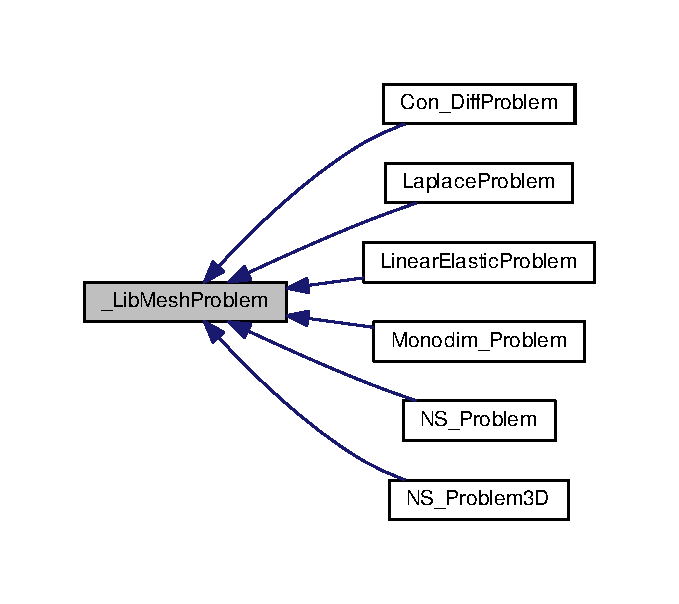
\includegraphics[width=326pt]{class___lib_mesh_problem__inherit__graph}
\end{center}
\end{figure}


Collaboration diagram for \-\_\-\-Lib\-Mesh\-Problem\-:\nopagebreak
\begin{figure}[H]
\begin{center}
\leavevmode
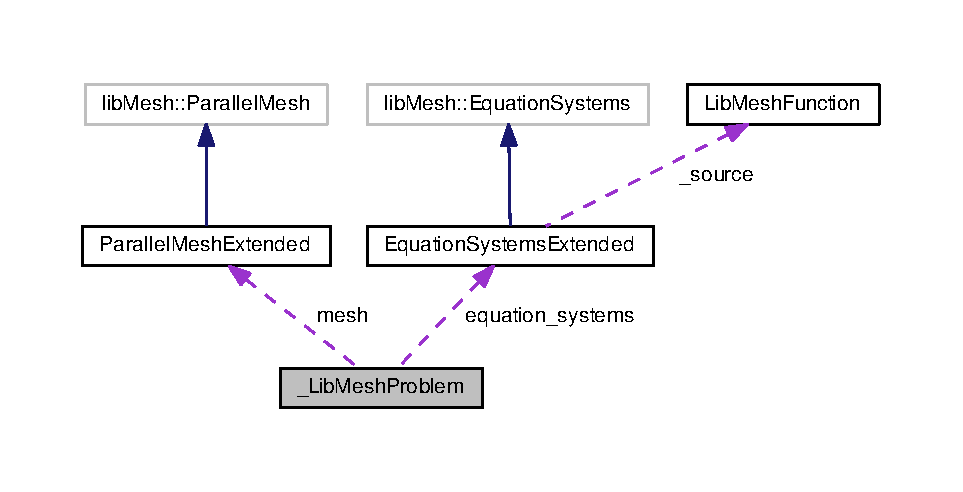
\includegraphics[width=350pt]{class___lib_mesh_problem__coll__graph}
\end{center}
\end{figure}
\subsection*{Public Member Functions}
\begin{DoxyCompactItemize}
\item 
\hypertarget{class___lib_mesh_problem_aa8b45f543865525921a0188cdb40c722}{{\bfseries \-\_\-\-Lib\-Mesh\-Problem} (const char $\ast$pb\-Name, int n\-Comp, M\-P\-I\-\_\-\-Comm comm)}\label{class___lib_mesh_problem_aa8b45f543865525921a0188cdb40c722}

\item 
\hypertarget{class___lib_mesh_problem_ab9d4af87f97b093870adc785f070a96a}{virtual void {\bfseries terminate} ()}\label{class___lib_mesh_problem_ab9d4af87f97b093870adc785f070a96a}

\item 
\hypertarget{class___lib_mesh_problem_acc417a3f26197a4abf46b4ea4a2ccdcb}{virtual void {\bfseries set\-Mesh} (const Para\-M\-E\-D\-M\-E\-M\-::\-M\-E\-D\-Coupling\-U\-Mesh $\ast$mesh)}\label{class___lib_mesh_problem_acc417a3f26197a4abf46b4ea4a2ccdcb}

\item 
\hypertarget{class___lib_mesh_problem_aa6a56c7bca6bf8b5bc8a5da7045280aa}{const \\*
Para\-M\-E\-D\-M\-E\-M\-::\-M\-E\-D\-Coupling\-U\-Mesh $\ast$ {\bfseries get\-Mesh} () const }\label{class___lib_mesh_problem_aa6a56c7bca6bf8b5bc8a5da7045280aa}

\item 
\hypertarget{class___lib_mesh_problem_a4dc21623bffc6471b6e8597e74d0fbaa}{virtual lib\-Mesh\-::boundary\-\_\-id\-\_\-type {\bfseries define\-Boundary} (const Para\-M\-E\-D\-M\-E\-M\-::\-M\-E\-D\-Coupling\-U\-Mesh $\ast$bc)}\label{class___lib_mesh_problem_a4dc21623bffc6471b6e8597e74d0fbaa}

\item 
\hypertarget{class___lib_mesh_problem_a26f77ccf7e7b55b67a1497c43b393629}{virtual void {\bfseries solve} ()}\label{class___lib_mesh_problem_a26f77ccf7e7b55b67a1497c43b393629}

\item 
\hypertarget{class___lib_mesh_problem_aa0d625e0ce00f1324b001060d1bd37c5}{virtual void {\bfseries set\-Analytic\-Source} (const char $\ast$f)}\label{class___lib_mesh_problem_aa0d625e0ce00f1324b001060d1bd37c5}

\item 
\hypertarget{class___lib_mesh_problem_aa14caed6e73a8c173454badc3d1fec54}{virtual void {\bfseries set\-Source} (const Para\-M\-E\-D\-M\-E\-M\-::\-M\-E\-D\-Coupling\-Field\-Double $\ast$f)}\label{class___lib_mesh_problem_aa14caed6e73a8c173454badc3d1fec54}

\item 
\hypertarget{class___lib_mesh_problem_a16072901cecfeb9bbd0b0d08fbfe57f9}{virtual void {\bfseries set\-Average\-Sources} (int n, double val\mbox{[}$\,$\mbox{]})}\label{class___lib_mesh_problem_a16072901cecfeb9bbd0b0d08fbfe57f9}

\item 
\hypertarget{class___lib_mesh_problem_a946fb7a10e983e72514e3425dad4c3e3}{virtual void {\bfseries set\-Boundary\-Condition\-Type} (int, const char $\ast$type\-B\-C)}\label{class___lib_mesh_problem_a946fb7a10e983e72514e3425dad4c3e3}

\item 
\hypertarget{class___lib_mesh_problem_adbbdfff37ef4e7b782158e149a34734a}{virtual void {\bfseries set\-Analytic\-Boundary\-Values} (int, const char $\ast$f)}\label{class___lib_mesh_problem_adbbdfff37ef4e7b782158e149a34734a}

\item 
\hypertarget{class___lib_mesh_problem_a557e861b6fa94257b6709f75326b7b36}{virtual void {\bfseries set\-Field\-Boundary\-Values} (int, const Para\-M\-E\-D\-M\-E\-M\-::\-M\-E\-D\-Coupling\-Field\-Double $\ast$f)}\label{class___lib_mesh_problem_a557e861b6fa94257b6709f75326b7b36}

\item 
\hypertarget{class___lib_mesh_problem_a40cf9bfb39fd30c9ba333125d5b0f1d1}{virtual \\*
Para\-M\-E\-D\-M\-E\-M\-::\-M\-E\-D\-Coupling\-Field\-Double $\ast$ {\bfseries get\-Output\-Field} (const char $\ast$v\-Name) const =0}\label{class___lib_mesh_problem_a40cf9bfb39fd30c9ba333125d5b0f1d1}

\item 
\hypertarget{class___lib_mesh_problem_a3f1ba458781b0786b964d307a1c9052d}{Para\-M\-E\-D\-M\-E\-M\-::\-M\-E\-D\-Coupling\-Field\-Double $\ast$ {\bfseries get\-Boundary\-Values} (const Para\-M\-E\-D\-M\-E\-M\-::\-M\-E\-D\-Coupling\-U\-Mesh $\ast$bc) const }\label{class___lib_mesh_problem_a3f1ba458781b0786b964d307a1c9052d}

\item 
\hypertarget{class___lib_mesh_problem_adabbbfc50e278f967b2f807c3c53efde}{Para\-M\-E\-D\-M\-E\-M\-::\-M\-E\-D\-Coupling\-Field\-Double $\ast$ {\bfseries get\-Values\-On\-Boundary} (int, const char $\ast$) const }\label{class___lib_mesh_problem_adabbbfc50e278f967b2f807c3c53efde}

\item 
\hypertarget{class___lib_mesh_problem_ae4cf3497851c96cb997aed6dbd6434df}{Para\-M\-E\-D\-M\-E\-M\-::\-M\-E\-D\-Coupling\-Field\-Double $\ast$ {\bfseries get\-Values\-On\-Boundary} (int, std\-::vector$<$ char $\ast$ $>$) const }\label{class___lib_mesh_problem_ae4cf3497851c96cb997aed6dbd6434df}

\item 
\hypertarget{class___lib_mesh_problem_a230e0d7521a755a4a71227212a8279f0}{Para\-M\-E\-D\-M\-E\-M\-::\-M\-E\-D\-Coupling\-Field\-Double $\ast$ {\bfseries get\-Values\-On\-Boundary\-\_\-nodes} (int, std\-::vector$<$ char $\ast$ $>$) const }\label{class___lib_mesh_problem_a230e0d7521a755a4a71227212a8279f0}

\end{DoxyCompactItemize}
\subsection*{Protected Member Functions}
\begin{DoxyCompactItemize}
\item 
\hypertarget{class___lib_mesh_problem_ad18da25656836fdeafa55fcec911cdc4}{virtual void {\bfseries \-\_\-init\-System} ()=0}\label{class___lib_mesh_problem_ad18da25656836fdeafa55fcec911cdc4}

\item 
\hypertarget{class___lib_mesh_problem_af4073a757108aa59b63182af50062e0b}{lib\-Mesh\-::\-System $\ast$ {\bfseries \-\_\-get\-Var\-Ids} (std\-::vector$<$ char $\ast$ $>$ name, std\-::vector$<$ int $>$ \&) const }\label{class___lib_mesh_problem_af4073a757108aa59b63182af50062e0b}

\item 
\hypertarget{class___lib_mesh_problem_aef5edc837a66d52055730d089d1a4689}{lib\-Mesh\-::\-System $\ast$ {\bfseries \-\_\-get\-Var\-Ids} (const char $\ast$name, std\-::vector$<$ int $>$ \&) const }\label{class___lib_mesh_problem_aef5edc837a66d52055730d089d1a4689}

\item 
\hypertarget{class___lib_mesh_problem_a24984c147004e33d7a00e9fe09d754d2}{Para\-M\-E\-D\-M\-E\-M\-::\-M\-E\-D\-Coupling\-Field\-Double $\ast$ {\bfseries \-\_\-get\-Output\-Field} (const char $\ast$v\-Name, Para\-M\-E\-D\-M\-E\-M\-::\-Type\-Of\-Field) const }\label{class___lib_mesh_problem_a24984c147004e33d7a00e9fe09d754d2}

\end{DoxyCompactItemize}
\subsection*{Protected Attributes}
\begin{DoxyCompactItemize}
\item 
\hypertarget{class___lib_mesh_problem_ab45902984281a4a6460443ae5ea80737}{M\-P\-I\-\_\-\-Comm {\bfseries \-\_\-comm}}\label{class___lib_mesh_problem_ab45902984281a4a6460443ae5ea80737}

\item 
\hypertarget{class___lib_mesh_problem_a4a12c20724ed9561bdaabdd1205548a1}{lib\-Mesh\-::\-Lib\-Mesh\-Init $\ast$ {\bfseries \-\_\-init\-Lib\-Mesh}}\label{class___lib_mesh_problem_a4a12c20724ed9561bdaabdd1205548a1}

\item 
\hypertarget{class___lib_mesh_problem_a6ea27959c2c72628bef4195991451948}{std\-::string {\bfseries problem\-Name}}\label{class___lib_mesh_problem_a6ea27959c2c72628bef4195991451948}

\item 
\hypertarget{class___lib_mesh_problem_ac48b158e95da1ecd9825ceb1200c566f}{const \\*
Para\-M\-E\-D\-M\-E\-M\-::\-M\-E\-D\-Coupling\-U\-Mesh $\ast$ {\bfseries med\-\_\-mesh}}\label{class___lib_mesh_problem_ac48b158e95da1ecd9825ceb1200c566f}

\item 
\hypertarget{class___lib_mesh_problem_ac094f4bbfb23d0a923fca0bbc6819a7c}{\hyperlink{class_parallel_mesh_extended}{Parallel\-Mesh\-Extended} $\ast$ {\bfseries mesh}}\label{class___lib_mesh_problem_ac094f4bbfb23d0a923fca0bbc6819a7c}

\item 
\hypertarget{class___lib_mesh_problem_a6ef56bdc17332a06789f3e7ea14bd8f6}{\hyperlink{class_equation_systems_extended}{Equation\-Systems\-Extended} $\ast$ {\bfseries equation\-\_\-systems}}\label{class___lib_mesh_problem_a6ef56bdc17332a06789f3e7ea14bd8f6}

\item 
\hypertarget{class___lib_mesh_problem_a40f55d4d5645515916e3825d742db0ca}{int {\bfseries \-\_\-n\-Comp}}\label{class___lib_mesh_problem_a40f55d4d5645515916e3825d742db0ca}

\item 
\hypertarget{class___lib_mesh_problem_a00366edec65284af72f89efbe1de02af}{std\-::map$<$ std\-::string, B\-C\-Type $>$ {\bfseries \-\_\-\-B\-C\-Types}}\label{class___lib_mesh_problem_a00366edec65284af72f89efbe1de02af}

\item 
\hypertarget{class___lib_mesh_problem_a652d4a40f5990654d7ad6cf92977a52c}{std\-::vector$<$ void($\ast$)(lib\-Mesh\-::\-Equation\-Systems \&)$>$ {\bfseries \-\_\-post\-\_\-processing\-\_\-functions}}\label{class___lib_mesh_problem_a652d4a40f5990654d7ad6cf92977a52c}

\end{DoxyCompactItemize}


The documentation for this class was generated from the following file\-:\begin{DoxyCompactItemize}
\item 
/homesd/msandro/software/femus/contrib/\-Libmesh\-\_\-cpp/libmesh\-\_\-problem/\-\_\-\-Lib\-Mesh\-Problem.\-h\end{DoxyCompactItemize}

\hypertarget{class_con___diff_problem}{\section{Con\-\_\-\-Diff\-Problem Class Reference}
\label{class_con___diff_problem}\index{Con\-\_\-\-Diff\-Problem@{Con\-\_\-\-Diff\-Problem}}
}


Inheritance diagram for Con\-\_\-\-Diff\-Problem\-:\nopagebreak
\begin{figure}[H]
\begin{center}
\leavevmode
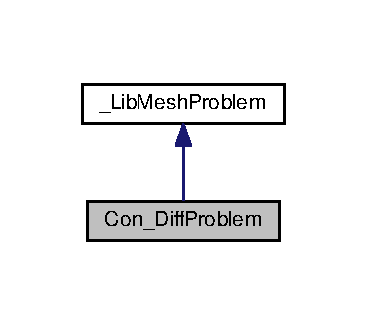
\includegraphics[width=176pt]{class_con___diff_problem__inherit__graph}
\end{center}
\end{figure}


Collaboration diagram for Con\-\_\-\-Diff\-Problem\-:\nopagebreak
\begin{figure}[H]
\begin{center}
\leavevmode
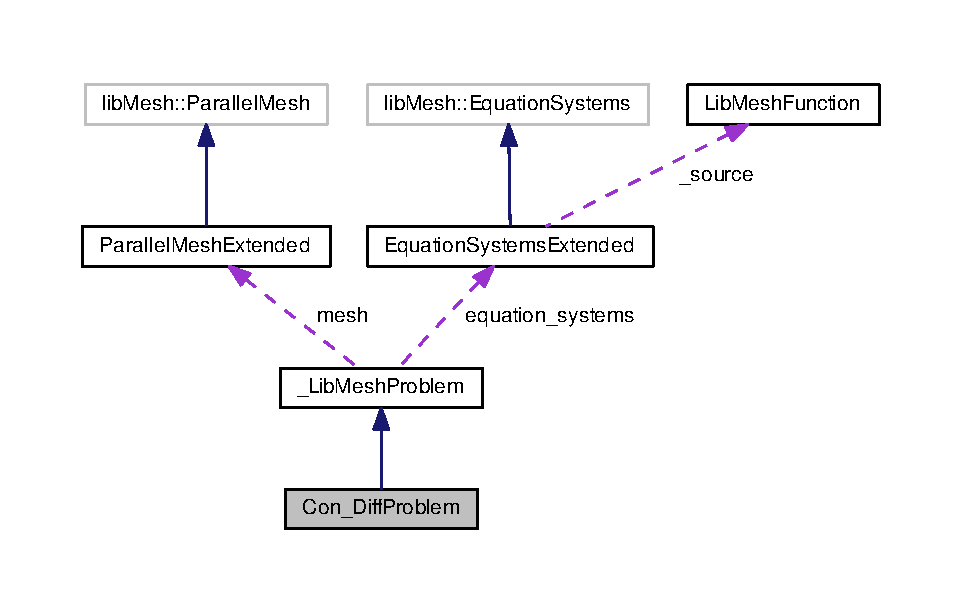
\includegraphics[width=350pt]{class_con___diff_problem__coll__graph}
\end{center}
\end{figure}
\subsection*{Public Member Functions}
\begin{DoxyCompactItemize}
\item 
\hypertarget{class_con___diff_problem_a55ec902fe07ef477b00e6c3baee5643d}{{\bfseries Con\-\_\-\-Diff\-Problem} (M\-P\-I\-\_\-\-Comm comm=M\-P\-I\-\_\-\-C\-O\-M\-M\-\_\-\-N\-U\-L\-L)}\label{class_con___diff_problem_a55ec902fe07ef477b00e6c3baee5643d}

\item 
\hypertarget{class_con___diff_problem_ac5abb233beb1a926c303a17532050057}{Para\-M\-E\-D\-M\-E\-M\-::\-M\-E\-D\-Coupling\-Field\-Double $\ast$ {\bfseries get\-Output\-Field} (const char $\ast$v\-Name) const }\label{class_con___diff_problem_ac5abb233beb1a926c303a17532050057}

\end{DoxyCompactItemize}
\subsection*{Protected Member Functions}
\begin{DoxyCompactItemize}
\item 
\hypertarget{class_con___diff_problem_a5087a6509c33681087461ceacc37c3bd}{void {\bfseries \-\_\-init\-System} ()}\label{class_con___diff_problem_a5087a6509c33681087461ceacc37c3bd}

\item 
\hypertarget{class_con___diff_problem_ac8072081699182d4f7189759e8e10e69}{void {\bfseries solve} ()}\label{class_con___diff_problem_ac8072081699182d4f7189759e8e10e69}

\end{DoxyCompactItemize}
\subsection*{Additional Inherited Members}


The documentation for this class was generated from the following file\-:\begin{DoxyCompactItemize}
\item 
/homesd/msandro/software/femus/contrib/\-Libmesh\-\_\-cpp/libmesh\-\_\-problem/Con\-\_\-\-Diff\-Problem.\-h\end{DoxyCompactItemize}

\hypertarget{class_debug}{\section{Debug Class Reference}
\label{class_debug}\index{Debug@{Debug}}
}


Inheritance diagram for Debug\-:\nopagebreak
\begin{figure}[H]
\begin{center}
\leavevmode
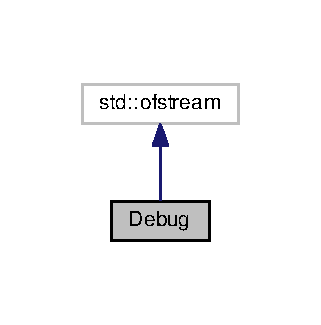
\includegraphics[width=154pt]{class_debug__inherit__graph}
\end{center}
\end{figure}


Collaboration diagram for Debug\-:\nopagebreak
\begin{figure}[H]
\begin{center}
\leavevmode
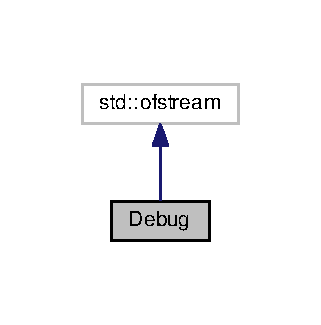
\includegraphics[width=154pt]{class_debug__coll__graph}
\end{center}
\end{figure}
\subsection*{Public Types}
\begin{DoxyCompactItemize}
\item 
\hypertarget{class_debug_a47958bd8d27052aae1d3ac2cb75b59a7}{typedef std\-::basic\-\_\-ostream\\*
$<$ char, std\-::char\-\_\-traits$<$ char $>$ $>$ {\bfseries Cout\-Type}}\label{class_debug_a47958bd8d27052aae1d3ac2cb75b59a7}

\item 
\hypertarget{class_debug_a30fab29155ac5ba0dd57c9b96dbe4fe6}{typedef Cout\-Type \&($\ast$ {\bfseries Standard\-End\-Line} )(Cout\-Type \&)}\label{class_debug_a30fab29155ac5ba0dd57c9b96dbe4fe6}

\end{DoxyCompactItemize}
\subsection*{Public Member Functions}
\begin{DoxyCompactItemize}
\item 
\hypertarget{class_debug_a20fb0d2a4f48ea6aba6c2303794837e0}{void {\bfseries open} (const char $\ast$file\-Name\-Prefix, M\-P\-I\-\_\-\-Comm comm=M\-P\-I\-\_\-\-C\-O\-M\-M\-\_\-\-N\-U\-L\-L)}\label{class_debug_a20fb0d2a4f48ea6aba6c2303794837e0}

\item 
\hypertarget{class_debug_a58a162758ce93f408bbaa70e3489e40f}{void {\bfseries position} (const char $\ast$, int)}\label{class_debug_a58a162758ce93f408bbaa70e3489e40f}

\item 
\hypertarget{class_debug_ae9967139f3da2c6e151265790eef1fc5}{\hyperlink{class_debug}{Debug} \& {\bfseries operator$<$$<$} (const lib\-Mesh\-::\-Node \&)}\label{class_debug_ae9967139f3da2c6e151265790eef1fc5}

\item 
\hypertarget{class_debug_a2e65ef865e0b52b6f6cb906b08df5a58}{\hyperlink{class_debug}{Debug} \& {\bfseries operator$<$$<$} (const lib\-Mesh\-::\-Elem \&)}\label{class_debug_a2e65ef865e0b52b6f6cb906b08df5a58}

\item 
\hypertarget{class_debug_a79184450d80f33bf78ac7d2fa9734492}{\hyperlink{class_debug}{Debug} \& {\bfseries operator$<$$<$} (Standard\-End\-Line manip)}\label{class_debug_a79184450d80f33bf78ac7d2fa9734492}

\item 
\hypertarget{class_debug_a81493a3be55e4a16bb152fc90a9dc56d}{{\footnotesize template$<$typename T $>$ }\\void {\bfseries array} (T $\ast$d, long n, long m, const char $\ast$s)}\label{class_debug_a81493a3be55e4a16bb152fc90a9dc56d}

\item 
\hypertarget{class_debug_a558bef398b4c903c758b8723a6dfcb81}{{\footnotesize template$<$typename T $>$ }\\void {\bfseries array} (std\-::vector$<$ T $\ast$ $>$ \&d)}\label{class_debug_a558bef398b4c903c758b8723a6dfcb81}

\item 
\hypertarget{class_debug_a43ac85062bc49da2b9a6317593daf244}{{\footnotesize template$<$typename T , typename U $>$ }\\void {\bfseries array} (const std\-::set$<$ T $\ast$, U $>$ \&d)}\label{class_debug_a43ac85062bc49da2b9a6317593daf244}

\item 
\hypertarget{class_debug_ad906eb2b4e449c9862fdabf09669b080}{{\footnotesize template$<$typename T $>$ }\\void {\bfseries array} (std\-::vector$<$ T $>$ $\ast$d, long n, long m, const char $\ast$s)}\label{class_debug_ad906eb2b4e449c9862fdabf09669b080}

\item 
\hypertarget{class_debug_a02bd26d249b025adb6f8e3c81c57ef39}{{\footnotesize template$<$typename T $>$ }\\void {\bfseries array} (std\-::vector$<$ std\-::vector$<$ T $>$ $\ast$ $>$ \&d, int n, std\-::vector$<$ int $>$ \&m, const char $\ast$s)}\label{class_debug_a02bd26d249b025adb6f8e3c81c57ef39}

\item 
\hypertarget{class_debug_a4c90d826f165cf6e73259eabbc455f9c}{void {\bfseries array} (const Para\-M\-E\-D\-M\-E\-M\-::\-Data\-Array\-Double $\ast$d, const char $\ast$s)}\label{class_debug_a4c90d826f165cf6e73259eabbc455f9c}

\item 
\hypertarget{class_debug_a348c9367ecbd8cb02deabaf7152652e4}{void {\bfseries array} (const Para\-M\-E\-D\-M\-E\-M\-::\-Data\-Array\-Int $\ast$d, const char $\ast$s)}\label{class_debug_a348c9367ecbd8cb02deabaf7152652e4}

\end{DoxyCompactItemize}
\subsection*{Protected Attributes}
\begin{DoxyCompactItemize}
\item 
\hypertarget{class_debug_a2f0df9c6e5cbc734691c50151538de9c}{bool {\bfseries \-\_\-prefix}}\label{class_debug_a2f0df9c6e5cbc734691c50151538de9c}

\end{DoxyCompactItemize}


The documentation for this class was generated from the following file\-:\begin{DoxyCompactItemize}
\item 
/homesd/msandro/software/femus/contrib/\-Libmesh\-\_\-cpp/\hyperlink{_debug_8h}{Debug.\-h}\end{DoxyCompactItemize}

\hypertarget{class_equation_systems_extended}{\section{Equation\-Systems\-Extended Class Reference}
\label{class_equation_systems_extended}\index{Equation\-Systems\-Extended@{Equation\-Systems\-Extended}}
}


Inheritance diagram for Equation\-Systems\-Extended\-:\nopagebreak
\begin{figure}[H]
\begin{center}
\leavevmode
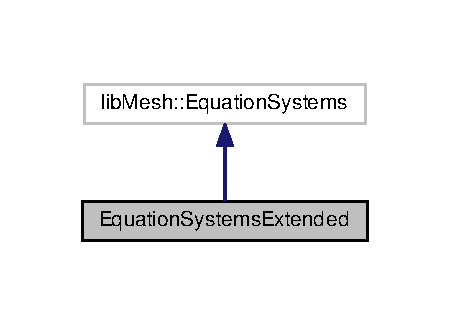
\includegraphics[width=216pt]{class_equation_systems_extended__inherit__graph}
\end{center}
\end{figure}


Collaboration diagram for Equation\-Systems\-Extended\-:\nopagebreak
\begin{figure}[H]
\begin{center}
\leavevmode
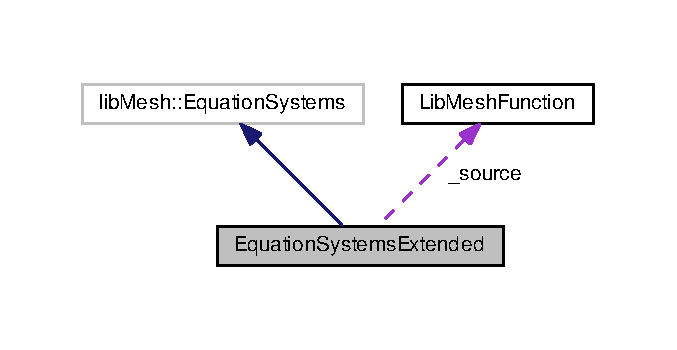
\includegraphics[width=325pt]{class_equation_systems_extended__coll__graph}
\end{center}
\end{figure}
\subsection*{Public Member Functions}
\begin{DoxyCompactItemize}
\item 
\hypertarget{class_equation_systems_extended_ac39a09a8c31cfdf406c512f97c8a621c}{{\bfseries Equation\-Systems\-Extended} (lib\-Mesh\-::\-Mesh\-Base \&mesh, int n\-Comp)}\label{class_equation_systems_extended_ac39a09a8c31cfdf406c512f97c8a621c}

\item 
\hypertarget{class_equation_systems_extended_a69834fd341bff79b73645507ba1b359c}{int {\bfseries get\-Number\-Of\-Components} () const }\label{class_equation_systems_extended_a69834fd341bff79b73645507ba1b359c}

\item 
\hypertarget{class_equation_systems_extended_a2a42b1a2930e2685a479922c1c6cb8a9}{void {\bfseries set\-Source} (const Para\-M\-E\-D\-M\-E\-M\-::\-M\-E\-D\-Coupling\-U\-Mesh $\ast$mesh, const char $\ast$s)}\label{class_equation_systems_extended_a2a42b1a2930e2685a479922c1c6cb8a9}

\item 
\hypertarget{class_equation_systems_extended_aeafd6d4c8fce5f31a26938a2c8660b70}{void {\bfseries erase\-Source} ()}\label{class_equation_systems_extended_aeafd6d4c8fce5f31a26938a2c8660b70}

\item 
\hypertarget{class_equation_systems_extended_a6fa1edb48c5ed6411d3e74b169445750}{\hyperlink{class_lib_mesh_function}{Lib\-Mesh\-Function} $\ast$ {\bfseries get\-Source} ()}\label{class_equation_systems_extended_a6fa1edb48c5ed6411d3e74b169445750}

\item 
\hypertarget{class_equation_systems_extended_aa5f0d1b7886f975cb3400c4185fcb5f3}{void {\bfseries set\-Average\-Sources} (int n\-\_\-\-Average\-Sources, double Average\mbox{[}$\,$\mbox{]})}\label{class_equation_systems_extended_aa5f0d1b7886f975cb3400c4185fcb5f3}

\item 
\hypertarget{class_equation_systems_extended_a92ae01b1dace5f3944e1a1d974dcbec2}{double {\bfseries get\-Average\-Sources} (int i)}\label{class_equation_systems_extended_a92ae01b1dace5f3944e1a1d974dcbec2}

\item 
\hypertarget{class_equation_systems_extended_a166f5f20a2e8f446cb21a2ddfc19ead3}{lib\-Mesh\-::boundary\-\_\-id\-\_\-type {\bfseries add\-B\-C} (const Para\-M\-E\-D\-M\-E\-M\-::\-M\-E\-D\-Coupling\-U\-Mesh $\ast$b)}\label{class_equation_systems_extended_a166f5f20a2e8f446cb21a2ddfc19ead3}

\item 
\hypertarget{class_equation_systems_extended_afa4ffe19c645d92af2aa4d4c7b799d07}{void {\bfseries set\-B\-C\-Type} (lib\-Mesh\-::boundary\-\_\-id\-\_\-type id, B\-C\-Type type)}\label{class_equation_systems_extended_afa4ffe19c645d92af2aa4d4c7b799d07}

\item 
\hypertarget{class_equation_systems_extended_ae1bbab9028311dc3a2ef2297905311b8}{void {\bfseries set\-B\-C} (lib\-Mesh\-::boundary\-\_\-id\-\_\-type id, const char $\ast$s)}\label{class_equation_systems_extended_ae1bbab9028311dc3a2ef2297905311b8}

\item 
\hypertarget{class_equation_systems_extended_a75fc3126e55a2e6969c14926ee896299}{void {\bfseries set\-B\-C} (lib\-Mesh\-::boundary\-\_\-id\-\_\-type id, const Para\-M\-E\-D\-M\-E\-M\-::\-M\-E\-D\-Coupling\-Field\-Double $\ast$f)}\label{class_equation_systems_extended_a75fc3126e55a2e6969c14926ee896299}

\item 
\hypertarget{class_equation_systems_extended_af214009f1b614348b2c667ca55738373}{void {\bfseries set\-Node\-B\-C} (lib\-Mesh\-::boundary\-\_\-id\-\_\-type id, const Para\-M\-E\-D\-M\-E\-M\-::\-M\-E\-D\-Coupling\-Field\-Double $\ast$f)}\label{class_equation_systems_extended_af214009f1b614348b2c667ca55738373}

\item 
\hypertarget{class_equation_systems_extended_a2d7a946924a8a4a4f477a448cbe836d7}{\hyperlink{class_lib_mesh_function}{Lib\-Mesh\-Function} $\ast$ {\bfseries get\-B\-C} (lib\-Mesh\-::boundary\-\_\-id\-\_\-type id)}\label{class_equation_systems_extended_a2d7a946924a8a4a4f477a448cbe836d7}

\item 
\hypertarget{class_equation_systems_extended_a232ed47ce6bc9c48f42c8a38ccbbe0fd}{B\-C\-Type {\bfseries get\-B\-C\-Type} (lib\-Mesh\-::boundary\-\_\-id\-\_\-type id)}\label{class_equation_systems_extended_a232ed47ce6bc9c48f42c8a38ccbbe0fd}

\item 
\hypertarget{class_equation_systems_extended_aadc09201591129a63422e12dbcb7c779}{void {\bfseries erase\-B\-C} (lib\-Mesh\-::boundary\-\_\-id\-\_\-type id)}\label{class_equation_systems_extended_aadc09201591129a63422e12dbcb7c779}

\end{DoxyCompactItemize}
\subsection*{Public Attributes}
\begin{DoxyCompactItemize}
\item 
\hypertarget{class_equation_systems_extended_a37c0c30082ee92fc8195969695d87474}{std\-::map\\*
$<$ lib\-Mesh\-::boundary\-\_\-id\-\_\-type, \\*
\hyperlink{class_lib_mesh_function}{Lib\-Mesh\-Function} $\ast$ $>$ {\bfseries \-\_\-bc}}\label{class_equation_systems_extended_a37c0c30082ee92fc8195969695d87474}

\item 
\hypertarget{class_equation_systems_extended_abe0bbb5dd4e66bb634d5e3003451d3b9}{std\-::map\\*
$<$ lib\-Mesh\-::boundary\-\_\-id\-\_\-type, \\*
B\-C\-Type $>$ {\bfseries \-\_\-bc\-\_\-type}}\label{class_equation_systems_extended_abe0bbb5dd4e66bb634d5e3003451d3b9}

\end{DoxyCompactItemize}
\subsection*{Protected Attributes}
\begin{DoxyCompactItemize}
\item 
\hypertarget{class_equation_systems_extended_aeeef0f52af137e0ae8021e7fb6989e2a}{int {\bfseries \-\_\-n\-Comp}}\label{class_equation_systems_extended_aeeef0f52af137e0ae8021e7fb6989e2a}

\item 
\hypertarget{class_equation_systems_extended_a5609a5a415dea40ff7264b6b53cf26b7}{\hyperlink{class_lib_mesh_function}{Lib\-Mesh\-Function} $\ast$ {\bfseries \-\_\-source}}\label{class_equation_systems_extended_a5609a5a415dea40ff7264b6b53cf26b7}

\item 
\hypertarget{class_equation_systems_extended_a0505b7fb4c30cafd27c60fe6687d15e3}{int {\bfseries \-\_\-n\-Average\-Sources}}\label{class_equation_systems_extended_a0505b7fb4c30cafd27c60fe6687d15e3}

\item 
\hypertarget{class_equation_systems_extended_abad40a2d66eb3c3fbef641e903e06b24}{double $\ast$ {\bfseries \-\_\-\-Average\-Sources}}\label{class_equation_systems_extended_abad40a2d66eb3c3fbef641e903e06b24}

\end{DoxyCompactItemize}


The documentation for this class was generated from the following file\-:\begin{DoxyCompactItemize}
\item 
/homesd/msandro/software/femus/contrib/\-Libmesh\-\_\-cpp/Equation\-Systems\-Extended.\-h\end{DoxyCompactItemize}

\hypertarget{class_laplace_problem}{\section{Laplace\-Problem Class Reference}
\label{class_laplace_problem}\index{Laplace\-Problem@{Laplace\-Problem}}
}


Inheritance diagram for Laplace\-Problem\-:\nopagebreak
\begin{figure}[H]
\begin{center}
\leavevmode
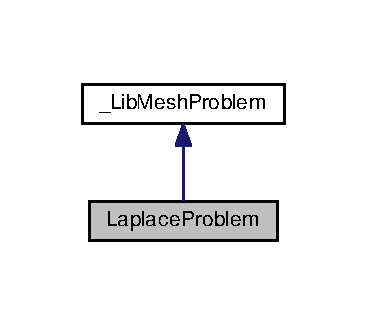
\includegraphics[width=176pt]{class_laplace_problem__inherit__graph}
\end{center}
\end{figure}


Collaboration diagram for Laplace\-Problem\-:\nopagebreak
\begin{figure}[H]
\begin{center}
\leavevmode
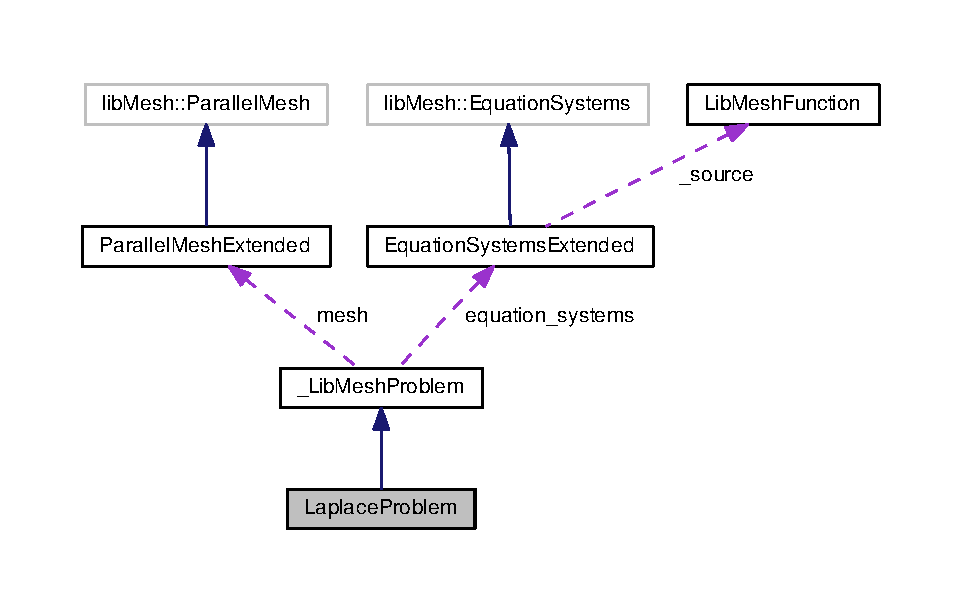
\includegraphics[width=350pt]{class_laplace_problem__coll__graph}
\end{center}
\end{figure}
\subsection*{Public Member Functions}
\begin{DoxyCompactItemize}
\item 
\hypertarget{class_laplace_problem_a28b5175097fa2fd12f5e9eb2ac9ff185}{{\bfseries Laplace\-Problem} (M\-P\-I\-\_\-\-Comm comm=M\-P\-I\-\_\-\-C\-O\-M\-M\-\_\-\-N\-U\-L\-L)}\label{class_laplace_problem_a28b5175097fa2fd12f5e9eb2ac9ff185}

\item 
\hypertarget{class_laplace_problem_aded2bdc3c30a256f6f8ac62ab29aef4b}{Para\-M\-E\-D\-M\-E\-M\-::\-M\-E\-D\-Coupling\-Field\-Double $\ast$ {\bfseries get\-Output\-Field} (const char $\ast$v\-Name) const }\label{class_laplace_problem_aded2bdc3c30a256f6f8ac62ab29aef4b}

\end{DoxyCompactItemize}
\subsection*{Protected Member Functions}
\begin{DoxyCompactItemize}
\item 
\hypertarget{class_laplace_problem_a3ce2b1fee526c7345b28ee856721c763}{void {\bfseries \-\_\-init\-System} ()}\label{class_laplace_problem_a3ce2b1fee526c7345b28ee856721c763}

\end{DoxyCompactItemize}
\subsection*{Additional Inherited Members}


The documentation for this class was generated from the following file\-:\begin{DoxyCompactItemize}
\item 
/homesd/msandro/software/femus/contrib/\-Libmesh\-\_\-cpp/libmesh\-\_\-problem/Laplace\-Problem.\-h\end{DoxyCompactItemize}

\hypertarget{class_l_i_b_m_e_s_h}{\section{L\-I\-B\-M\-E\-S\-H Class Reference}
\label{class_l_i_b_m_e_s_h}\index{L\-I\-B\-M\-E\-S\-H@{L\-I\-B\-M\-E\-S\-H}}
}


Collaboration diagram for L\-I\-B\-M\-E\-S\-H\-:\nopagebreak
\begin{figure}[H]
\begin{center}
\leavevmode
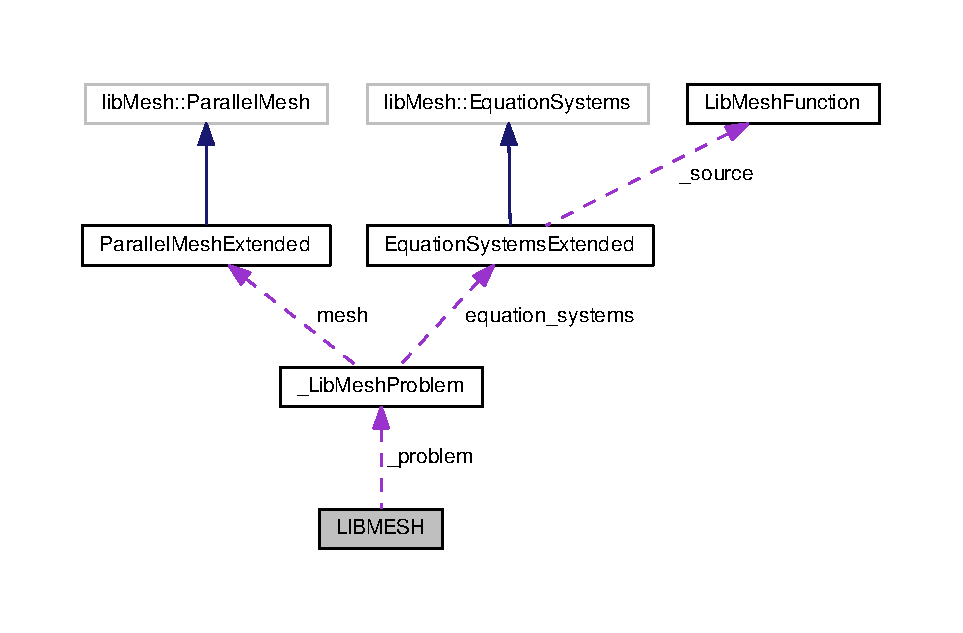
\includegraphics[width=350pt]{class_l_i_b_m_e_s_h__coll__graph}
\end{center}
\end{figure}
\subsection*{Classes}
\begin{DoxyCompactItemize}
\item 
struct \hyperlink{struct_l_i_b_m_e_s_h_1_1s_b_c}{s\-B\-C}
\end{DoxyCompactItemize}
\subsection*{Public Member Functions}
\begin{DoxyCompactItemize}
\item 
\hypertarget{class_l_i_b_m_e_s_h_a884f0cd9f294da8e7a23d3e03a8b6260}{{\bfseries L\-I\-B\-M\-E\-S\-H} (M\-P\-I\-\_\-\-Comm comm)}\label{class_l_i_b_m_e_s_h_a884f0cd9f294da8e7a23d3e03a8b6260}

\item 
\hypertarget{class_l_i_b_m_e_s_h_a4ebee9e21f12098cdcc50a7cc87c70b4}{void {\bfseries terminate} ()}\label{class_l_i_b_m_e_s_h_a4ebee9e21f12098cdcc50a7cc87c70b4}

\item 
\hypertarget{class_l_i_b_m_e_s_h_a9ffabbac5606f42ebaf2286eaadc1ac5}{void {\bfseries set\-Type} (const std\-::string \&pb\-Name)}\label{class_l_i_b_m_e_s_h_a9ffabbac5606f42ebaf2286eaadc1ac5}

\item 
\hypertarget{class_l_i_b_m_e_s_h_a0e16b3aa46db4ee9986eafe20e6080dd}{void {\bfseries set\-Mesh} (const std\-::string \&mesh\-File\-Name)}\label{class_l_i_b_m_e_s_h_a0e16b3aa46db4ee9986eafe20e6080dd}

\item 
\hypertarget{class_l_i_b_m_e_s_h_af12649c692b3e81ece14fae8767b7d79}{void {\bfseries solve} ()}\label{class_l_i_b_m_e_s_h_af12649c692b3e81ece14fae8767b7d79}

\item 
\hypertarget{class_l_i_b_m_e_s_h_a9241ce2d728502e34491e08441d7e69d}{Para\-M\-E\-D\-M\-E\-M\-::\-M\-E\-D\-Coupling\-Field\-Double $\ast$ {\bfseries get\-Output\-Field} (const std\-::string \&v\-Name) const }\label{class_l_i_b_m_e_s_h_a9241ce2d728502e34491e08441d7e69d}

\item 
\hypertarget{class_l_i_b_m_e_s_h_aae9f756e18bbc1840a0fce89c7fdd698}{void {\bfseries save\-Output\-Field} (const std\-::string \&v\-Name, const std\-::string \&prefix) const }\label{class_l_i_b_m_e_s_h_aae9f756e18bbc1840a0fce89c7fdd698}

\item 
\hypertarget{class_l_i_b_m_e_s_h_a78890b3c164cf0f7077e3039246a8587}{void {\bfseries set\-Source} (const Para\-M\-E\-D\-M\-E\-M\-::\-M\-E\-D\-Coupling\-Field\-Double $\ast$f)}\label{class_l_i_b_m_e_s_h_a78890b3c164cf0f7077e3039246a8587}

\item 
\hypertarget{class_l_i_b_m_e_s_h_ac81b0e8d508151e4b5ae7c23ac062d73}{void {\bfseries set\-Analytic\-Source} (const std\-::string \&f)}\label{class_l_i_b_m_e_s_h_ac81b0e8d508151e4b5ae7c23ac062d73}

\item 
\hypertarget{class_l_i_b_m_e_s_h_affe723f2d372b86e17b38128e7d043e7}{void {\bfseries set\-Average\-Sources} (int n, double val\mbox{[}$\,$\mbox{]})}\label{class_l_i_b_m_e_s_h_affe723f2d372b86e17b38128e7d043e7}

\item 
\hypertarget{class_l_i_b_m_e_s_h_a1c5b0fb11e684d38022e266910e50068}{std\-::vector$<$ std\-::string $>$ {\bfseries get\-Boundary\-Names} ()}\label{class_l_i_b_m_e_s_h_a1c5b0fb11e684d38022e266910e50068}

\item 
\hypertarget{class_l_i_b_m_e_s_h_a3bc61a5336af51535ac176dfb922f686}{std\-::string {\bfseries get\-Boundary\-Name} (int i)}\label{class_l_i_b_m_e_s_h_a3bc61a5336af51535ac176dfb922f686}

\item 
\hypertarget{class_l_i_b_m_e_s_h_a1ceb20870251b53bc3d6db5cc526527a}{void {\bfseries set\-Analytic\-Boundary\-Values} (const std\-::string \&name, const std\-::string \&type\-B\-C, const std\-::string \&f)}\label{class_l_i_b_m_e_s_h_a1ceb20870251b53bc3d6db5cc526527a}

\item 
\hypertarget{class_l_i_b_m_e_s_h_a7df5ad4fd176aa449c400c27ed668c27}{void {\bfseries set\-Field\-Boundary\-Values} (const std\-::string \&name, const std\-::string \&bc\-Type, const Para\-M\-E\-D\-M\-E\-M\-::\-M\-E\-D\-Coupling\-Field\-Double $\ast$bc\-Field)}\label{class_l_i_b_m_e_s_h_a7df5ad4fd176aa449c400c27ed668c27}

\item 
\hypertarget{class_l_i_b_m_e_s_h_af54e016f79a070f14d9c371ef7053e6c}{Para\-M\-E\-D\-M\-E\-M\-::\-M\-E\-D\-Coupling\-Field\-Double $\ast$ {\bfseries get\-Values\-On\-Boundary} (const std\-::string \&name, const std\-::string \&v\-Name) const }\label{class_l_i_b_m_e_s_h_af54e016f79a070f14d9c371ef7053e6c}

\item 
\hypertarget{class_l_i_b_m_e_s_h_a47823d380756e39ea0d2dba9561e13d3}{Para\-M\-E\-D\-M\-E\-M\-::\-M\-E\-D\-Coupling\-Field\-Double $\ast$ {\bfseries get\-Values\-On\-Boundary} (const std\-::string \&name, std\-::vector$<$ char $\ast$ $>$ v\-Name) const }\label{class_l_i_b_m_e_s_h_a47823d380756e39ea0d2dba9561e13d3}

\item 
\hypertarget{class_l_i_b_m_e_s_h_a4eebed17ef5c78efce759b42a527aca9}{Para\-M\-E\-D\-M\-E\-M\-::\-M\-E\-D\-Coupling\-Field\-Double $\ast$ {\bfseries get\-Values\-On\-Boundary\-\_\-nodes} (const std\-::string \&name, std\-::vector$<$ char $\ast$ $>$) const }\label{class_l_i_b_m_e_s_h_a4eebed17ef5c78efce759b42a527aca9}

\item 
\hypertarget{class_l_i_b_m_e_s_h_a8608739ac966d63fd803cd77ae4e1a1f}{Para\-M\-E\-D\-M\-E\-M\-::\-M\-E\-D\-Coupling\-Field\-Double $\ast$ {\bfseries get\-Input\-Field\-Template} (const std\-::string \&name)}\label{class_l_i_b_m_e_s_h_a8608739ac966d63fd803cd77ae4e1a1f}

\item 
\hypertarget{class_l_i_b_m_e_s_h_addbb8f89d4a02d0e23cde7965a65158b}{void {\bfseries set\-Debug\-File} (const std\-::string \&s)}\label{class_l_i_b_m_e_s_h_addbb8f89d4a02d0e23cde7965a65158b}

\item 
\hypertarget{class_l_i_b_m_e_s_h_ad33629ec2a02e86d8a9b0ad2cd2f3bd3}{void {\bfseries end\-Debug} ()}\label{class_l_i_b_m_e_s_h_ad33629ec2a02e86d8a9b0ad2cd2f3bd3}

\end{DoxyCompactItemize}
\subsection*{Protected Member Functions}
\begin{DoxyCompactItemize}
\item 
\hypertarget{class_l_i_b_m_e_s_h_aae41ff7a833629b5cbcf67cff328a6b6}{void {\bfseries set\-B\-C\-Type} (const std\-::string \&bc\-Name, const std\-::string \&type\-B\-C)}\label{class_l_i_b_m_e_s_h_aae41ff7a833629b5cbcf67cff328a6b6}

\item 
\hypertarget{class_l_i_b_m_e_s_h_a84c031a0f038ed3d72d7fd8a27596913}{void {\bfseries set\-Mesh} (const Para\-M\-E\-D\-M\-E\-M\-::\-M\-E\-D\-Coupling\-U\-Mesh $\ast$m)}\label{class_l_i_b_m_e_s_h_a84c031a0f038ed3d72d7fd8a27596913}

\item 
\hypertarget{class_l_i_b_m_e_s_h_a0d034a75893e66fb1eefb97d3f696f71}{int {\bfseries define\-Boundary} (const Para\-M\-E\-D\-M\-E\-M\-::\-M\-E\-D\-Coupling\-U\-Mesh $\ast$support)}\label{class_l_i_b_m_e_s_h_a0d034a75893e66fb1eefb97d3f696f71}

\item 
\hypertarget{class_l_i_b_m_e_s_h_af9e3ba09f53d09b1047649b274a2b54a}{int {\bfseries search\-Boundary\-Condition} (const std\-::string \&) const }\label{class_l_i_b_m_e_s_h_af9e3ba09f53d09b1047649b274a2b54a}

\item 
\hypertarget{class_l_i_b_m_e_s_h_aceb23ee70e4758befd12fde103156dbc}{void {\bfseries set\-Analytic\-B\-C\-Values} (const std\-::string \&bc\-Name, const std\-::string \&f)}\label{class_l_i_b_m_e_s_h_aceb23ee70e4758befd12fde103156dbc}

\item 
\hypertarget{class_l_i_b_m_e_s_h_a53e8192426ef6ec098f4a0f966b0fe2c}{void {\bfseries set\-Field\-B\-C\-Values} (const std\-::string \&bc\-Name, const Para\-M\-E\-D\-M\-E\-M\-::\-M\-E\-D\-Coupling\-Field\-Double $\ast$f)}\label{class_l_i_b_m_e_s_h_a53e8192426ef6ec098f4a0f966b0fe2c}

\end{DoxyCompactItemize}
\subsection*{Protected Attributes}
\begin{DoxyCompactItemize}
\item 
\hypertarget{class_l_i_b_m_e_s_h_a672bcec2de95c12d86d594f54bfb6e55}{M\-P\-I\-\_\-\-Comm {\bfseries \-\_\-comm}}\label{class_l_i_b_m_e_s_h_a672bcec2de95c12d86d594f54bfb6e55}

\item 
\hypertarget{class_l_i_b_m_e_s_h_a836c17ddc2b45f517af79325175bcb38}{\hyperlink{class___lib_mesh_problem}{\-\_\-\-Lib\-Mesh\-Problem} $\ast$ {\bfseries \-\_\-problem}}\label{class_l_i_b_m_e_s_h_a836c17ddc2b45f517af79325175bcb38}

\item 
\hypertarget{class_l_i_b_m_e_s_h_a73ffe80e881ed92baa61c7063420ebc6}{Para\-M\-E\-D\-M\-E\-M\-::\-M\-E\-D\-Coupling\-U\-Mesh $\ast$ {\bfseries \-\_\-mesh}}\label{class_l_i_b_m_e_s_h_a73ffe80e881ed92baa61c7063420ebc6}

\item 
\hypertarget{class_l_i_b_m_e_s_h_a95ac038769a7a6f8e76423c99e04929a}{std\-::vector$<$ \hyperlink{struct_l_i_b_m_e_s_h_1_1s_b_c}{s\-B\-C} $>$ {\bfseries \-\_\-bc}}\label{class_l_i_b_m_e_s_h_a95ac038769a7a6f8e76423c99e04929a}

\item 
\hypertarget{class_l_i_b_m_e_s_h_a979cb8ef6d2003c3c038c63de18c9e85}{bool {\bfseries \-\_\-local\-\_\-\-M\-P\-I\-\_\-\-Init}}\label{class_l_i_b_m_e_s_h_a979cb8ef6d2003c3c038c63de18c9e85}

\end{DoxyCompactItemize}


The documentation for this class was generated from the following file\-:\begin{DoxyCompactItemize}
\item 
/homesd/msandro/software/femus/contrib/\-Libmesh\-\_\-cpp/L\-I\-B\-M\-E\-S\-H.\-h\end{DoxyCompactItemize}

\hypertarget{class_lib_mesh_function}{\section{Lib\-Mesh\-Function Class Reference}
\label{class_lib_mesh_function}\index{Lib\-Mesh\-Function@{Lib\-Mesh\-Function}}
}
\subsection*{Public Member Functions}
\begin{DoxyCompactItemize}
\item 
\hypertarget{class_lib_mesh_function_a8c22f2e9dc4e255dfc8888e38fe9d688}{void {\bfseries eval} (int, std\-::vector$<$ double $>$ \&v)}\label{class_lib_mesh_function_a8c22f2e9dc4e255dfc8888e38fe9d688}

\item 
\hypertarget{class_lib_mesh_function_a9df4401cfbd9c27ace6dcdd441a18787}{void {\bfseries eval} (int, int, std\-::vector$<$ double $>$ \&v)}\label{class_lib_mesh_function_a9df4401cfbd9c27ace6dcdd441a18787}

\item 
\hypertarget{class_lib_mesh_function_a0778d03df178e86de022c893c1b1a397}{void {\bfseries set\-Support} (const lib\-Mesh\-::\-Mesh\-Base $\ast$mesh, const Para\-M\-E\-D\-M\-E\-M\-::\-M\-E\-D\-Coupling\-U\-Mesh $\ast$support)}\label{class_lib_mesh_function_a0778d03df178e86de022c893c1b1a397}

\item 
\hypertarget{class_lib_mesh_function_a4a9515b721c933221d8ad9e68bc59930}{void {\bfseries set\-Code} (const char $\ast$code, int n\-Comp)}\label{class_lib_mesh_function_a4a9515b721c933221d8ad9e68bc59930}

\item 
\hypertarget{class_lib_mesh_function_a4ed4ba8e51d30b060c926edbdc2cb956}{void {\bfseries set\-Field} (const Para\-M\-E\-D\-M\-E\-M\-::\-M\-E\-D\-Coupling\-Field\-Double $\ast$f)}\label{class_lib_mesh_function_a4ed4ba8e51d30b060c926edbdc2cb956}

\item 
\hypertarget{class_lib_mesh_function_ade0bad107a585542200cdce50396f93e}{std\-::map$<$ std\-::pair$<$ int, int $>$\\*
, int $>$ \& {\bfseries Face\-I\-D} ()}\label{class_lib_mesh_function_ade0bad107a585542200cdce50396f93e}

\item 
\hypertarget{class_lib_mesh_function_a9333f7d3da708de7a14637389c40b75d}{std\-::map$<$ int, int $>$ \& {\bfseries Node\-I\-D} ()}\label{class_lib_mesh_function_a9333f7d3da708de7a14637389c40b75d}

\item 
\hypertarget{class_lib_mesh_function_a455f565d4bcedad79a3ece4bc38cb213}{std\-::map$<$ int, int $>$ \& {\bfseries Elem\-I\-D} ()}\label{class_lib_mesh_function_a455f565d4bcedad79a3ece4bc38cb213}

\item 
\hypertarget{class_lib_mesh_function_a89398c781ae98e1130281232cae85585}{Para\-M\-E\-D\-M\-E\-M\-::\-M\-E\-D\-Coupling\-Field\-Double $\ast$ {\bfseries get\-Field} (const char $\ast$v\-Name)}\label{class_lib_mesh_function_a89398c781ae98e1130281232cae85585}

\item 
\hypertarget{class_lib_mesh_function_acbf42955775e5024568eb53ee7d3f92f}{const \\*
Para\-M\-E\-D\-M\-E\-M\-::\-M\-E\-D\-Coupling\-U\-Mesh $\ast$ {\bfseries get\-Support} ()}\label{class_lib_mesh_function_acbf42955775e5024568eb53ee7d3f92f}

\item 
\hypertarget{class_lib_mesh_function_ab382d27c50b41b0cbe41a134b98fa74c}{void {\bfseries print\-On} (std\-::ostream \&out) const }\label{class_lib_mesh_function_ab382d27c50b41b0cbe41a134b98fa74c}

\end{DoxyCompactItemize}
\subsection*{Protected Attributes}
\begin{DoxyCompactItemize}
\item 
\hypertarget{class_lib_mesh_function_ad39808f78a545b8b838318402d25cb14}{const lib\-Mesh\-::\-Mesh\-Base $\ast$ {\bfseries \-\_\-mesh}}\label{class_lib_mesh_function_ad39808f78a545b8b838318402d25cb14}

\item 
\hypertarget{class_lib_mesh_function_a74d20b871fdfae3e2b159f7a757fbccd}{const \\*
Para\-M\-E\-D\-M\-E\-M\-::\-M\-E\-D\-Coupling\-U\-Mesh $\ast$ {\bfseries \-\_\-support}}\label{class_lib_mesh_function_a74d20b871fdfae3e2b159f7a757fbccd}

\item 
\hypertarget{class_lib_mesh_function_a1102eeaea5166fa6e5db44e708ee9aa5}{Para\-M\-E\-D\-M\-E\-M\-::\-M\-E\-D\-Coupling\-Field\-Double $\ast$ {\bfseries \-\_\-f}}\label{class_lib_mesh_function_a1102eeaea5166fa6e5db44e708ee9aa5}

\item 
\hypertarget{class_lib_mesh_function_ab387e7ad966a62774124231d3206aaa9}{std\-::map$<$ int, int $>$ {\bfseries \-\_\-node\-I\-D}}\label{class_lib_mesh_function_ab387e7ad966a62774124231d3206aaa9}

\item 
\hypertarget{class_lib_mesh_function_a900c549c6c4d0e62ddb974b0cf0d380f}{std\-::map$<$ std\-::pair$<$ int, int $>$\\*
, int $>$ {\bfseries \-\_\-face\-I\-D}}\label{class_lib_mesh_function_a900c549c6c4d0e62ddb974b0cf0d380f}

\item 
\hypertarget{class_lib_mesh_function_aeafaef87a7a08e730d65712efb0ceb54}{std\-::map$<$ int, int $>$ {\bfseries \-\_\-elem\-I\-D}}\label{class_lib_mesh_function_aeafaef87a7a08e730d65712efb0ceb54}

\end{DoxyCompactItemize}


The documentation for this class was generated from the following file\-:\begin{DoxyCompactItemize}
\item 
/homesd/msandro/software/femus/contrib/\-Libmesh\-\_\-cpp/Lib\-Mesh\-Function.\-h\end{DoxyCompactItemize}

\hypertarget{class_linear_elastic_problem}{\section{Linear\-Elastic\-Problem Class Reference}
\label{class_linear_elastic_problem}\index{Linear\-Elastic\-Problem@{Linear\-Elastic\-Problem}}
}


Inheritance diagram for Linear\-Elastic\-Problem\-:\nopagebreak
\begin{figure}[H]
\begin{center}
\leavevmode
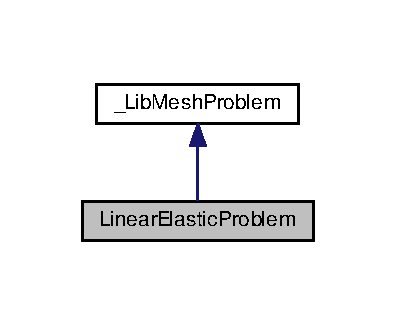
\includegraphics[width=190pt]{class_linear_elastic_problem__inherit__graph}
\end{center}
\end{figure}


Collaboration diagram for Linear\-Elastic\-Problem\-:\nopagebreak
\begin{figure}[H]
\begin{center}
\leavevmode
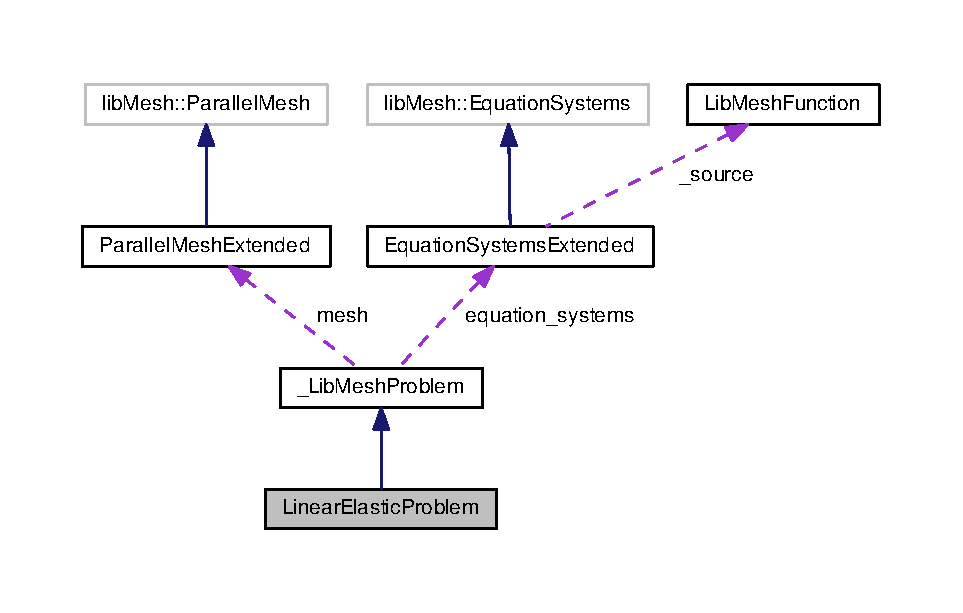
\includegraphics[width=350pt]{class_linear_elastic_problem__coll__graph}
\end{center}
\end{figure}
\subsection*{Public Member Functions}
\begin{DoxyCompactItemize}
\item 
\hypertarget{class_linear_elastic_problem_a7ab0868a3958a95308efc3fb60ce6484}{{\bfseries Linear\-Elastic\-Problem} (M\-P\-I\-\_\-\-Comm comm=M\-P\-I\-\_\-\-C\-O\-M\-M\-\_\-\-N\-U\-L\-L)}\label{class_linear_elastic_problem_a7ab0868a3958a95308efc3fb60ce6484}

\item 
\hypertarget{class_linear_elastic_problem_a51c3ca5ecd1279d797c81ea00adc0005}{Para\-M\-E\-D\-M\-E\-M\-::\-M\-E\-D\-Coupling\-Field\-Double $\ast$ {\bfseries get\-Output\-Field} (const char $\ast$v\-Name) const }\label{class_linear_elastic_problem_a51c3ca5ecd1279d797c81ea00adc0005}

\end{DoxyCompactItemize}
\subsection*{Protected Member Functions}
\begin{DoxyCompactItemize}
\item 
\hypertarget{class_linear_elastic_problem_a9fcc48fd002d9d7d48ff91c8e9d5acd9}{void {\bfseries \-\_\-init\-System} ()}\label{class_linear_elastic_problem_a9fcc48fd002d9d7d48ff91c8e9d5acd9}

\item 
\hypertarget{class_linear_elastic_problem_a098b7d34a0808f7f6c4d76292d86a0d0}{void {\bfseries \-\_\-get\-\_\-stresses} (int i\-Var, std\-::vector$<$ double $>$ \&v)}\label{class_linear_elastic_problem_a098b7d34a0808f7f6c4d76292d86a0d0}

\end{DoxyCompactItemize}
\subsection*{Additional Inherited Members}


The documentation for this class was generated from the following file\-:\begin{DoxyCompactItemize}
\item 
/homesd/msandro/software/femus/contrib/\-Libmesh\-\_\-cpp/libmesh\-\_\-problem/Linear\-Elastic\-Problem.\-h\end{DoxyCompactItemize}

\hypertarget{class_monodim___problem}{\section{Monodim\-\_\-\-Problem Class Reference}
\label{class_monodim___problem}\index{Monodim\-\_\-\-Problem@{Monodim\-\_\-\-Problem}}
}


Inheritance diagram for Monodim\-\_\-\-Problem\-:\nopagebreak
\begin{figure}[H]
\begin{center}
\leavevmode
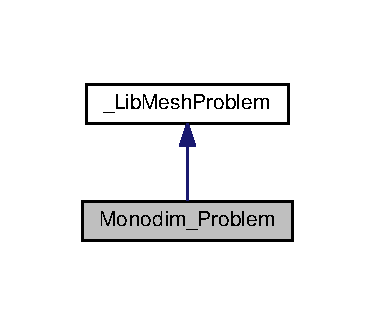
\includegraphics[width=180pt]{class_monodim___problem__inherit__graph}
\end{center}
\end{figure}


Collaboration diagram for Monodim\-\_\-\-Problem\-:\nopagebreak
\begin{figure}[H]
\begin{center}
\leavevmode
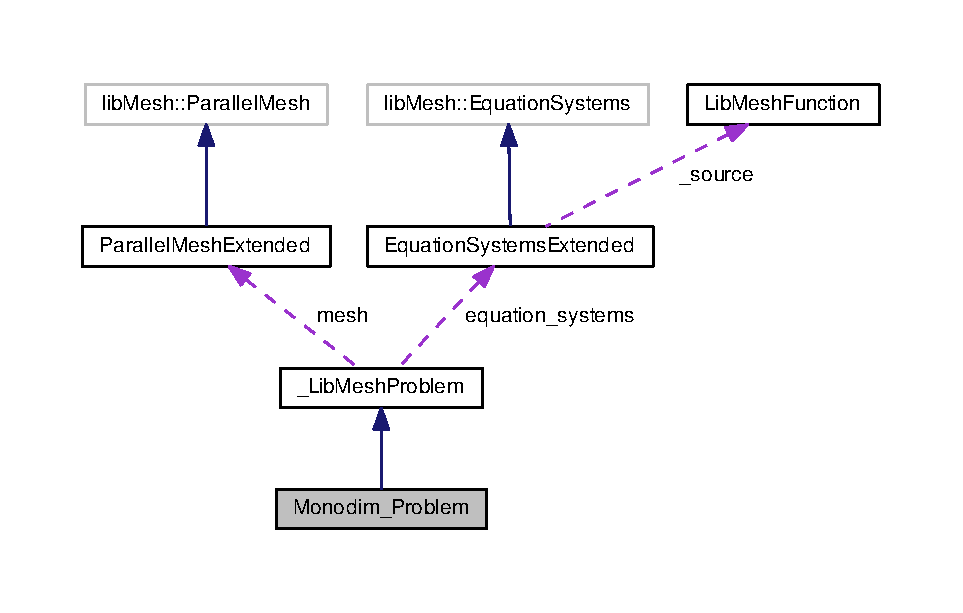
\includegraphics[width=350pt]{class_monodim___problem__coll__graph}
\end{center}
\end{figure}
\subsection*{Public Member Functions}
\begin{DoxyCompactItemize}
\item 
\hypertarget{class_monodim___problem_aa10ea73f10a8522864285623e56bbd9d}{{\bfseries Monodim\-\_\-\-Problem} (M\-P\-I\-\_\-\-Comm comm=M\-P\-I\-\_\-\-C\-O\-M\-M\-\_\-\-N\-U\-L\-L)}\label{class_monodim___problem_aa10ea73f10a8522864285623e56bbd9d}

\item 
\hypertarget{class_monodim___problem_aa2010ed59798e7bf539fb26a5197f2cb}{Para\-M\-E\-D\-M\-E\-M\-::\-M\-E\-D\-Coupling\-Field\-Double $\ast$ {\bfseries get\-Output\-Field} (const char $\ast$v\-Name) const }\label{class_monodim___problem_aa2010ed59798e7bf539fb26a5197f2cb}

\end{DoxyCompactItemize}
\subsection*{Protected Member Functions}
\begin{DoxyCompactItemize}
\item 
\hypertarget{class_monodim___problem_a1a46815fc044d21fd69eeeeafde045df}{void {\bfseries \-\_\-init\-System} ()}\label{class_monodim___problem_a1a46815fc044d21fd69eeeeafde045df}

\item 
\hypertarget{class_monodim___problem_a90b1fcc9ab7e572b493ad239b2c6983d}{void {\bfseries solve} ()}\label{class_monodim___problem_a90b1fcc9ab7e572b493ad239b2c6983d}

\end{DoxyCompactItemize}
\subsection*{Additional Inherited Members}


The documentation for this class was generated from the following file\-:\begin{DoxyCompactItemize}
\item 
/homesd/msandro/software/femus/contrib/\-Libmesh\-\_\-cpp/libmesh\-\_\-problem/Monodim\-Problem.\-h\end{DoxyCompactItemize}

\hypertarget{structnode_compare}{\section{node\-Compare Struct Reference}
\label{structnode_compare}\index{node\-Compare@{node\-Compare}}
}
\subsection*{Public Member Functions}
\begin{DoxyCompactItemize}
\item 
\hypertarget{structnode_compare_af9460e8163ea400d84620bccc033639d}{bool {\bfseries operator()} (const lib\-Mesh\-::\-Node $\ast$p, const lib\-Mesh\-::\-Node $\ast$q) const }\label{structnode_compare_af9460e8163ea400d84620bccc033639d}

\end{DoxyCompactItemize}
\subsection*{Static Public Attributes}
\begin{DoxyCompactItemize}
\item 
\hypertarget{structnode_compare_a66792864fbc3fe22e785a68b246451ce}{static const double {\bfseries eps}}\label{structnode_compare_a66792864fbc3fe22e785a68b246451ce}

\end{DoxyCompactItemize}


The documentation for this struct was generated from the following file\-:\begin{DoxyCompactItemize}
\item 
/homesd/msandro/software/femus/contrib/\-Libmesh\-\_\-cpp/Lib\-Mesh\-Util.\-h\end{DoxyCompactItemize}

\hypertarget{class_node_ext}{\section{Node\-Ext Class Reference}
\label{class_node_ext}\index{Node\-Ext@{Node\-Ext}}
}


Inheritance diagram for Node\-Ext\-:\nopagebreak
\begin{figure}[H]
\begin{center}
\leavevmode
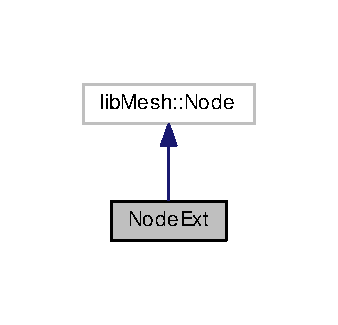
\includegraphics[width=162pt]{class_node_ext__inherit__graph}
\end{center}
\end{figure}


Collaboration diagram for Node\-Ext\-:\nopagebreak
\begin{figure}[H]
\begin{center}
\leavevmode
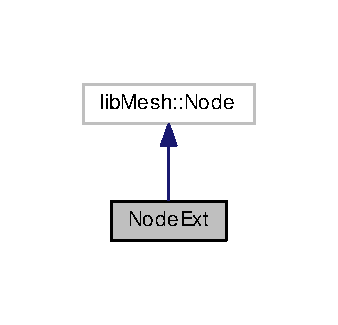
\includegraphics[width=162pt]{class_node_ext__coll__graph}
\end{center}
\end{figure}
\subsection*{Public Member Functions}
\begin{DoxyCompactItemize}
\item 
\hypertarget{class_node_ext_a7077383f48c3c23b8eee43b561f466c1}{{\bfseries Node\-Ext} (const lib\-Mesh\-::\-Point \&n, int id, int id2)}\label{class_node_ext_a7077383f48c3c23b8eee43b561f466c1}

\item 
\hypertarget{class_node_ext_a9c55ed76c5901c4ab499b4e950c4d2ea}{int \& {\bfseries set\-\_\-id2} ()}\label{class_node_ext_a9c55ed76c5901c4ab499b4e950c4d2ea}

\item 
\hypertarget{class_node_ext_ad0a2baff589e7bcefec4487ea494218e}{int {\bfseries id2} () const }\label{class_node_ext_ad0a2baff589e7bcefec4487ea494218e}

\end{DoxyCompactItemize}
\subsection*{Protected Attributes}
\begin{DoxyCompactItemize}
\item 
\hypertarget{class_node_ext_abeeca035ab4e1bd1d12ef555c3314c53}{int {\bfseries \-\_\-id2}}\label{class_node_ext_abeeca035ab4e1bd1d12ef555c3314c53}

\end{DoxyCompactItemize}


The documentation for this class was generated from the following file\-:\begin{DoxyCompactItemize}
\item 
/homesd/msandro/software/femus/contrib/\-Libmesh\-\_\-cpp/Lib\-Mesh\-Util.\-h\end{DoxyCompactItemize}

\hypertarget{class_n_s___problem}{\section{N\-S\-\_\-\-Problem Class Reference}
\label{class_n_s___problem}\index{N\-S\-\_\-\-Problem@{N\-S\-\_\-\-Problem}}
}


Inheritance diagram for N\-S\-\_\-\-Problem\-:\nopagebreak
\begin{figure}[H]
\begin{center}
\leavevmode
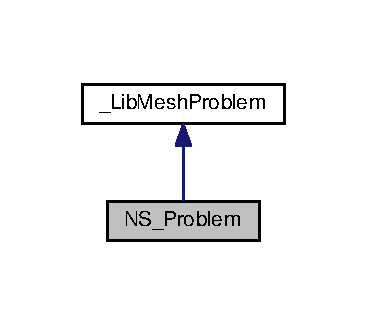
\includegraphics[width=176pt]{class_n_s___problem__inherit__graph}
\end{center}
\end{figure}


Collaboration diagram for N\-S\-\_\-\-Problem\-:\nopagebreak
\begin{figure}[H]
\begin{center}
\leavevmode
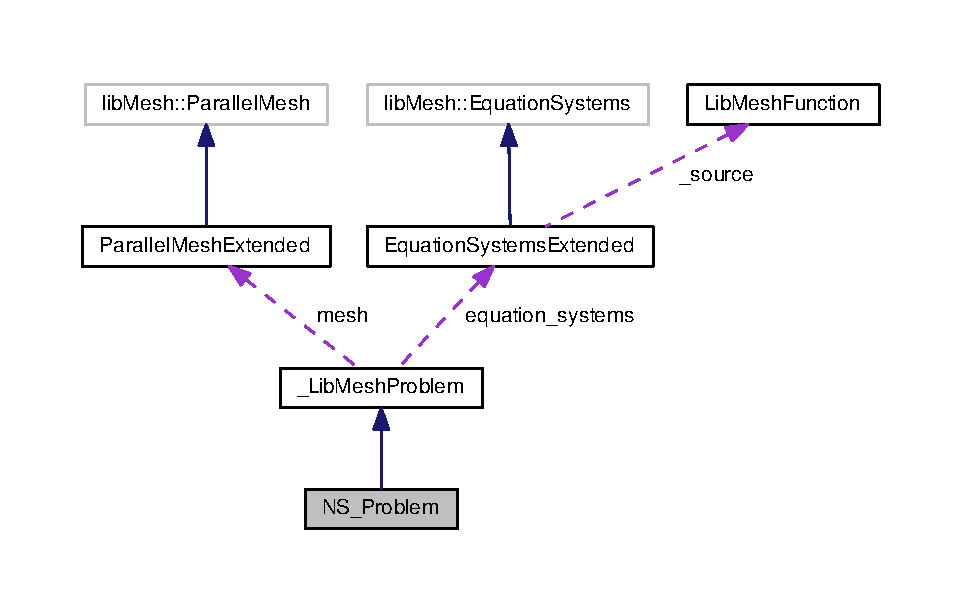
\includegraphics[width=350pt]{class_n_s___problem__coll__graph}
\end{center}
\end{figure}
\subsection*{Public Member Functions}
\begin{DoxyCompactItemize}
\item 
\hypertarget{class_n_s___problem_a64926f3eaa48618d5e96b76e9c3e8c01}{{\bfseries N\-S\-\_\-\-Problem} (M\-P\-I\-\_\-\-Comm comm=M\-P\-I\-\_\-\-C\-O\-M\-M\-\_\-\-N\-U\-L\-L)}\label{class_n_s___problem_a64926f3eaa48618d5e96b76e9c3e8c01}

\item 
\hypertarget{class_n_s___problem_a93c104e0d749884e447315ca3ac23a25}{Para\-M\-E\-D\-M\-E\-M\-::\-M\-E\-D\-Coupling\-Field\-Double $\ast$ {\bfseries get\-Output\-Field} (const char $\ast$v\-Name) const }\label{class_n_s___problem_a93c104e0d749884e447315ca3ac23a25}

\end{DoxyCompactItemize}
\subsection*{Protected Member Functions}
\begin{DoxyCompactItemize}
\item 
\hypertarget{class_n_s___problem_a6ebc7696f40b10db61d600ff76650c79}{void {\bfseries \-\_\-init\-System} ()}\label{class_n_s___problem_a6ebc7696f40b10db61d600ff76650c79}

\item 
\hypertarget{class_n_s___problem_a2a89eee5839c48d2deffee37b9aafd4a}{void {\bfseries solve} ()}\label{class_n_s___problem_a2a89eee5839c48d2deffee37b9aafd4a}

\end{DoxyCompactItemize}
\subsection*{Additional Inherited Members}


The documentation for this class was generated from the following file\-:\begin{DoxyCompactItemize}
\item 
/homesd/msandro/software/femus/contrib/\-Libmesh\-\_\-cpp/libmesh\-\_\-problem/N\-S\-\_\-\-Problem.\-h\end{DoxyCompactItemize}

\hypertarget{class_n_s___problem3_d}{\section{N\-S\-\_\-\-Problem3\-D Class Reference}
\label{class_n_s___problem3_d}\index{N\-S\-\_\-\-Problem3\-D@{N\-S\-\_\-\-Problem3\-D}}
}


Inheritance diagram for N\-S\-\_\-\-Problem3\-D\-:\nopagebreak
\begin{figure}[H]
\begin{center}
\leavevmode
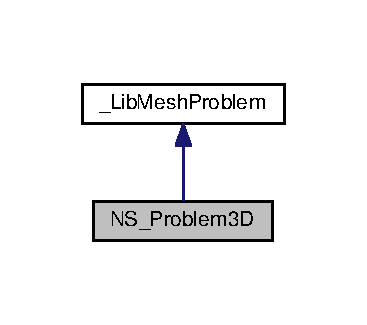
\includegraphics[width=176pt]{class_n_s___problem3_d__inherit__graph}
\end{center}
\end{figure}


Collaboration diagram for N\-S\-\_\-\-Problem3\-D\-:\nopagebreak
\begin{figure}[H]
\begin{center}
\leavevmode
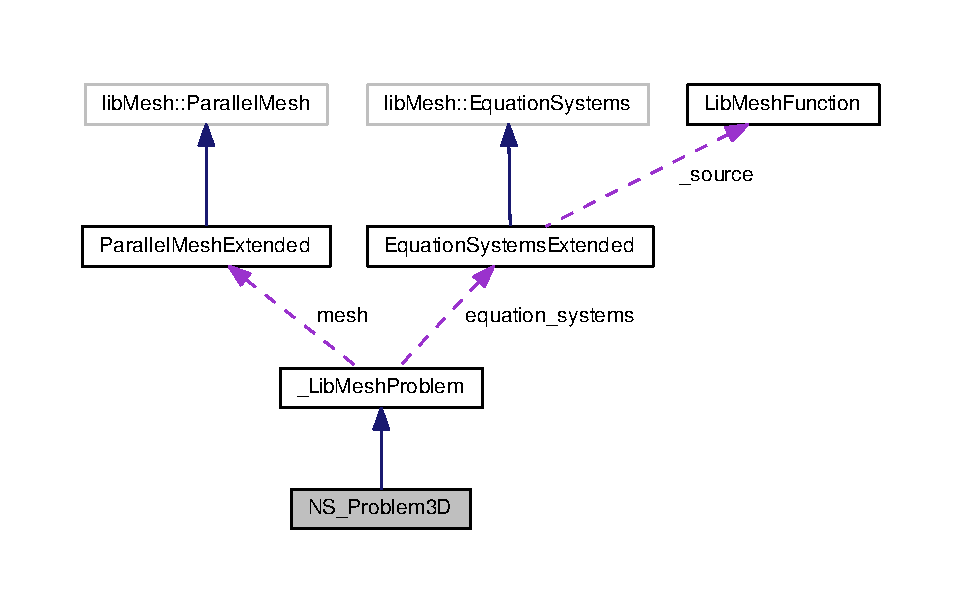
\includegraphics[width=350pt]{class_n_s___problem3_d__coll__graph}
\end{center}
\end{figure}
\subsection*{Public Member Functions}
\begin{DoxyCompactItemize}
\item 
\hypertarget{class_n_s___problem3_d_aa5a745dbba07071135a65050f222dfb3}{{\bfseries N\-S\-\_\-\-Problem3\-D} (M\-P\-I\-\_\-\-Comm comm=M\-P\-I\-\_\-\-C\-O\-M\-M\-\_\-\-N\-U\-L\-L)}\label{class_n_s___problem3_d_aa5a745dbba07071135a65050f222dfb3}

\item 
\hypertarget{class_n_s___problem3_d_a27c720f9ccc76f28a22fd4d069e2234c}{Para\-M\-E\-D\-M\-E\-M\-::\-M\-E\-D\-Coupling\-Field\-Double $\ast$ {\bfseries get\-Output\-Field} (const char $\ast$v\-Name) const }\label{class_n_s___problem3_d_a27c720f9ccc76f28a22fd4d069e2234c}

\end{DoxyCompactItemize}
\subsection*{Protected Member Functions}
\begin{DoxyCompactItemize}
\item 
\hypertarget{class_n_s___problem3_d_aa75a9508c7c6d2681444278e4fc85d3c}{void {\bfseries \-\_\-init\-System} ()}\label{class_n_s___problem3_d_aa75a9508c7c6d2681444278e4fc85d3c}

\item 
\hypertarget{class_n_s___problem3_d_a7f0d1aeec7fec9cf33289344452ff3f3}{void {\bfseries solve} ()}\label{class_n_s___problem3_d_a7f0d1aeec7fec9cf33289344452ff3f3}

\end{DoxyCompactItemize}
\subsection*{Additional Inherited Members}


The documentation for this class was generated from the following file\-:\begin{DoxyCompactItemize}
\item 
/homesd/msandro/software/femus/contrib/\-Libmesh\-\_\-cpp/libmesh\-\_\-problem/N\-S\-\_\-\-Problem3\-D.\-h\end{DoxyCompactItemize}

\hypertarget{class_parallel_mesh_extended}{\section{Parallel\-Mesh\-Extended Class Reference}
\label{class_parallel_mesh_extended}\index{Parallel\-Mesh\-Extended@{Parallel\-Mesh\-Extended}}
}


Inheritance diagram for Parallel\-Mesh\-Extended\-:\nopagebreak
\begin{figure}[H]
\begin{center}
\leavevmode
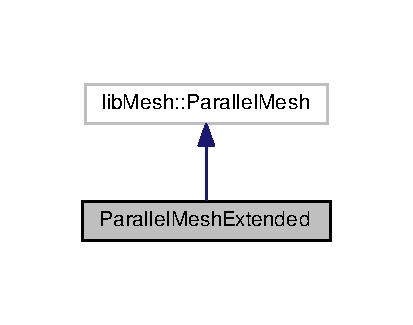
\includegraphics[width=198pt]{class_parallel_mesh_extended__inherit__graph}
\end{center}
\end{figure}


Collaboration diagram for Parallel\-Mesh\-Extended\-:\nopagebreak
\begin{figure}[H]
\begin{center}
\leavevmode
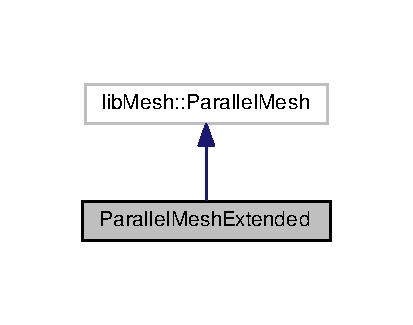
\includegraphics[width=198pt]{class_parallel_mesh_extended__coll__graph}
\end{center}
\end{figure}
\subsection*{Public Member Functions}
\begin{DoxyCompactItemize}
\item 
\hypertarget{class_parallel_mesh_extended_a0be992f122b572d6f5bf1f2079152c88}{{\bfseries Parallel\-Mesh\-Extended} (const Para\-M\-E\-D\-M\-E\-M\-::\-M\-E\-D\-Coupling\-U\-Mesh \&mesh, M\-P\-I\-\_\-\-Comm comm=M\-P\-I\-\_\-\-C\-O\-M\-M\-\_\-\-N\-U\-L\-L)}\label{class_parallel_mesh_extended_a0be992f122b572d6f5bf1f2079152c88}

\item 
\hypertarget{class_parallel_mesh_extended_a4ffaee6ac14a4010be015c8962a2b9b5}{const std\-::vector$<$ int $>$ \& {\bfseries get\-Node\-I\-D} () const }\label{class_parallel_mesh_extended_a4ffaee6ac14a4010be015c8962a2b9b5}

\item 
\hypertarget{class_parallel_mesh_extended_a51dcfe18578035f50f470e012217dd79}{const std\-::vector$<$ int $>$ \& {\bfseries get\-Proc\-I\-D} () const }\label{class_parallel_mesh_extended_a51dcfe18578035f50f470e012217dd79}

\item 
\hypertarget{class_parallel_mesh_extended_adcdc784bda5416960f835b5541846e0a}{const std\-::vector$<$ int $>$ \& {\bfseries get\-Elem\-I\-D} () const }\label{class_parallel_mesh_extended_adcdc784bda5416960f835b5541846e0a}

\item 
\hypertarget{class_parallel_mesh_extended_abde3b507dc64b44a463f33b851c0bc5d}{int {\bfseries mesh\-Dimension} ()}\label{class_parallel_mesh_extended_abde3b507dc64b44a463f33b851c0bc5d}

\end{DoxyCompactItemize}
\subsection*{Protected Attributes}
\begin{DoxyCompactItemize}
\item 
\hypertarget{class_parallel_mesh_extended_aeb9adf72dc239202ddec8b928fdc9c7d}{const \\*
Para\-M\-E\-D\-M\-E\-M\-::\-M\-E\-D\-Coupling\-U\-Mesh \& {\bfseries \-\_\-mesh}}\label{class_parallel_mesh_extended_aeb9adf72dc239202ddec8b928fdc9c7d}

\item 
\hypertarget{class_parallel_mesh_extended_ac8507f7fb4ecede1bd3885c5ba22aa35}{M\-P\-I\-\_\-\-Comm {\bfseries \-\_\-comm}}\label{class_parallel_mesh_extended_ac8507f7fb4ecede1bd3885c5ba22aa35}

\item 
\hypertarget{class_parallel_mesh_extended_ae2c38384c21cc833eaff1f4d64141811}{std\-::vector$<$ int $>$ {\bfseries \-\_\-node\-\_\-id}}\label{class_parallel_mesh_extended_ae2c38384c21cc833eaff1f4d64141811}

\item 
\hypertarget{class_parallel_mesh_extended_a76ebcd5d238e56d2783a4dcd56fd61ff}{std\-::vector$<$ int $>$ {\bfseries \-\_\-proc\-\_\-id}}\label{class_parallel_mesh_extended_a76ebcd5d238e56d2783a4dcd56fd61ff}

\item 
\hypertarget{class_parallel_mesh_extended_aeedaefe4710c9088edb9a9b1672fe6ae}{std\-::vector$<$ int $>$ {\bfseries \-\_\-elem\-\_\-id}}\label{class_parallel_mesh_extended_aeedaefe4710c9088edb9a9b1672fe6ae}

\item 
\hypertarget{class_parallel_mesh_extended_aa9281577930c18e5b2767c361fa4f9fa}{int {\bfseries \-\_\-mesh\-Dim}}\label{class_parallel_mesh_extended_aa9281577930c18e5b2767c361fa4f9fa}

\end{DoxyCompactItemize}


The documentation for this class was generated from the following file\-:\begin{DoxyCompactItemize}
\item 
/homesd/msandro/software/femus/contrib/\-Libmesh\-\_\-cpp/Parallel\-Mesh\-Extended.\-h\end{DoxyCompactItemize}

\hypertarget{struct_l_i_b_m_e_s_h_1_1s_b_c}{\section{L\-I\-B\-M\-E\-S\-H\-:\-:s\-B\-C Struct Reference}
\label{struct_l_i_b_m_e_s_h_1_1s_b_c}\index{L\-I\-B\-M\-E\-S\-H\-::s\-B\-C@{L\-I\-B\-M\-E\-S\-H\-::s\-B\-C}}
}
\subsection*{Public Attributes}
\begin{DoxyCompactItemize}
\item 
\hypertarget{struct_l_i_b_m_e_s_h_1_1s_b_c_a3d5075ed0d26b7d782d37440a914b038}{int {\bfseries id}}\label{struct_l_i_b_m_e_s_h_1_1s_b_c_a3d5075ed0d26b7d782d37440a914b038}

\item 
\hypertarget{struct_l_i_b_m_e_s_h_1_1s_b_c_a73a5a5bb10149dc38dddcc6702181579}{std\-::string {\bfseries name}}\label{struct_l_i_b_m_e_s_h_1_1s_b_c_a73a5a5bb10149dc38dddcc6702181579}

\item 
\hypertarget{struct_l_i_b_m_e_s_h_1_1s_b_c_ad299f44348472939d112cec6968d7e3e}{Para\-M\-E\-D\-M\-E\-M\-::\-M\-E\-D\-Coupling\-U\-Mesh $\ast$ {\bfseries support}}\label{struct_l_i_b_m_e_s_h_1_1s_b_c_ad299f44348472939d112cec6968d7e3e}

\end{DoxyCompactItemize}


The documentation for this struct was generated from the following file\-:\begin{DoxyCompactItemize}
\item 
/homesd/msandro/software/femus/contrib/\-Libmesh\-\_\-cpp/L\-I\-B\-M\-E\-S\-H.\-h\end{DoxyCompactItemize}

\hypertarget{class_timer}{\section{Timer Class Reference}
\label{class_timer}\index{Timer@{Timer}}
}
\subsection*{Public Member Functions}
\begin{DoxyCompactItemize}
\item 
\hypertarget{class_timer_a3a8b5272198d029779dc9302a54305a8}{void {\bfseries start} ()}\label{class_timer_a3a8b5272198d029779dc9302a54305a8}

\item 
\hypertarget{class_timer_a7a0f15257db9fa349a43042d3d28349b}{double {\bfseries elapsed} ()}\label{class_timer_a7a0f15257db9fa349a43042d3d28349b}

\item 
\hypertarget{class_timer_a0289effad7b573c508bc27e405900a23}{void {\bfseries pause} ()}\label{class_timer_a0289effad7b573c508bc27e405900a23}

\item 
\hypertarget{class_timer_a4ac55a73bb3431db9d4d2fd70ae9a2e8}{void {\bfseries resume} ()}\label{class_timer_a4ac55a73bb3431db9d4d2fd70ae9a2e8}

\end{DoxyCompactItemize}


The documentation for this class was generated from the following file\-:\begin{DoxyCompactItemize}
\item 
/homesd/msandro/software/femus/contrib/\-Libmesh\-\_\-cpp/Timer.\-h\end{DoxyCompactItemize}

\chapter{File Documentation}
\hypertarget{_debug_8h}{\section{/homesd/msandro/software/femus/contrib/\-Libmesh\-\_\-cpp/\-Debug.h File Reference}
\label{_debug_8h}\index{/homesd/msandro/software/femus/contrib/\-Libmesh\-\_\-cpp/\-Debug.\-h@{/homesd/msandro/software/femus/contrib/\-Libmesh\-\_\-cpp/\-Debug.\-h}}
}


definition of the \hyperlink{class_debug}{Debug} class, used to write text output in a different file for each process in a multi-\/processes run  


{\ttfamily \#include $<$mpi.\-h$>$}\\*
{\ttfamily \#include $<$fstream$>$}\\*
{\ttfamily \#include $<$iomanip$>$}\\*
{\ttfamily \#include $<$vector$>$}\\*
{\ttfamily \#include $<$set$>$}\\*
{\ttfamily \#include \char`\"{}M\-E\-D\-Coupling\-Mem\-Array.\-hxx\char`\"{}}\\*
Include dependency graph for Debug.\-h\-:\nopagebreak
\begin{figure}[H]
\begin{center}
\leavevmode
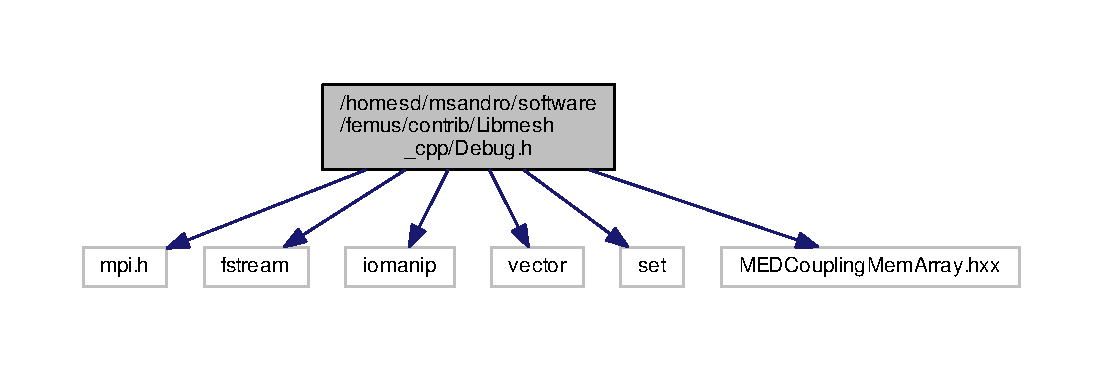
\includegraphics[width=350pt]{_debug_8h__incl}
\end{center}
\end{figure}
This graph shows which files directly or indirectly include this file\-:\nopagebreak
\begin{figure}[H]
\begin{center}
\leavevmode
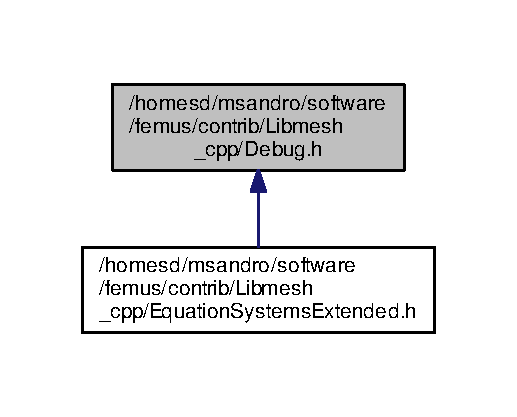
\includegraphics[width=248pt]{_debug_8h__dep__incl}
\end{center}
\end{figure}
\subsection*{Classes}
\begin{DoxyCompactItemize}
\item 
class \hyperlink{class_debug}{Debug}
\end{DoxyCompactItemize}
\subsection*{Macros}
\begin{DoxyCompactItemize}
\item 
\hypertarget{_debug_8h_ad9adfdc2e97918fe6ca23e1dffa67771}{\#define {\bfseries f\-Debug\-Pos}~f\-Debug.\-position(\-\_\-\-\_\-\-F\-I\-L\-E\-\_\-\-\_\-, \-\_\-\-\_\-\-L\-I\-N\-E\-\_\-\-\_\-); f\-Debug}\label{_debug_8h_ad9adfdc2e97918fe6ca23e1dffa67771}

\end{DoxyCompactItemize}
\subsection*{Variables}
\begin{DoxyCompactItemize}
\item 
\hypertarget{_debug_8h_aeb66465fc00fa9b489fce443ce6e9c36}{\hyperlink{class_debug}{Debug} {\bfseries f\-Debug}}\label{_debug_8h_aeb66465fc00fa9b489fce443ce6e9c36}

\end{DoxyCompactItemize}


\subsection{Detailed Description}
definition of the \hyperlink{class_debug}{Debug} class, used to write text output in a different file for each process in a multi-\/processes run \begin{DoxyAuthor}{Author}
Marc Tajchman (\href{mailto:marc.tajchman@cea.fr}{\tt marc.\-tajchman@cea.\-fr})
\end{DoxyAuthor}
\begin{DoxyDate}{Date}
2/12/2011 
\end{DoxyDate}

%--- End generated contents ---

% Index
\newpage
\phantomsection
\addcontentsline{toc}{part}{Index}
\printindex

\end{document}
